%% =============================================================================
%% Adaptive Orchestration of Learning Modalities for Embodied Agents on Edge
%% Hardware: A Survey
%% Target journal: IEEE Transactions on Neural Networks and Learning Systems
%% Template: IEEEtran (journal mode), IEEE reference style (IEEEtran.bst).
%% Compile: pdflatex main; bibtex main; pdflatex main; pdflatex main
%% =============================================================================
\documentclass[journal]{IEEEtran}
\usepackage{cite}
\usepackage{amsmath,amssymb,amsfonts}
\usepackage{graphicx}
\usepackage{booktabs}
\usepackage{array}
\usepackage{textcomp}
\usepackage{xcolor}
\usepackage{url}
\usepackage[hidelinks]{hyperref}
%% [FILL: ...] marks text the authors must complete before submission.
\newcommand{\fillin}[1]{{\color{red}\bfseries [FILL: #1]}}
\hyphenation{op-tical net-works semi-conduc-tor}

\begin{document}
\title{Adaptive Orchestration of Learning Modalities for Embodied Agents on Edge Hardware: A Survey}

%% ---------------------------------------------------------------------------
%% AUTHORS -- replace the placeholders. IEEE requires full names, membership
%% grades (if any), affiliations in the \thanks footnote, and biographies.
%% ---------------------------------------------------------------------------
\author{Firstname~Lastname,~\IEEEmembership{Student Member,~IEEE,}
        and~Second~Author,~\IEEEmembership{Member,~IEEE}%
\thanks{F. Lastname and S. Author are with the Department of ..., Institution, City, Country (e-mail: author@institution.edu).}%
\thanks{Manuscript received Month DD, 2026; revised Month DD, 2026.}}

\markboth{IEEE Transactions on Neural Networks and Learning Systems}%
{Lastname \MakeLowercase{\textit{et al.}}: Adaptive Orchestration of Learning Modalities on Edge Hardware}

\maketitle

\begin{abstract}
Low-cost robots are increasingly expected to perceive, learn from demonstration, improve through reinforcement, and recover from faults on the robot itself, without a cloud connection. Each of these learning modalities has matured separately, and large language models (LLMs) and vision--language--action (VLA) models now offer ways to plan over them. What is missing is a principled account of how an embodied agent should decide which modality to invoke, how much computation to spend, and how far to trust the result. This survey reviews 180 works that bear on this question, spanning LLM planners, VLA models, uncertainty quantification, reinforcement, imitation and meta-learning, fault recovery, uncertainty fusion, on-device continual learning, mixture-of-experts and adaptive computation, low-cost hardware, and safe learning. We organize the literature around four modalities, each paired with a confidence signal: epistemic uncertainty for perception, policy variance for reinforcement learning, behavioral fidelity for imitation, and recovery success for fault adaptation. Every work is graded on a six-level evidence scale. The components exist separately, but no published system composes heterogeneous learning modalities under a learned, uncertainty-aware, compute-budgeted orchestrator on edge hardware, and most capable models are too large for a 4-GB single-board computer. An illustrative simulation shows that routing on miscalibrated confidences lowers success from 0.85 to 0.81 at equal cost, and that recalibration restores it. We formalize orchestration as budget-constrained, confidence-driven routing and identify open challenges in cross-modality calibration, training while acting, and the safety of self-modifying learners.
\end{abstract}

\begin{IEEEkeywords}
Adaptive computation, edge computing, embodied agents, large language models, meta-learning, mixture of experts, robot learning, uncertainty quantification.
\end{IEEEkeywords}


\section{Introduction}\label{sec:intro}

\subsection{Adaptive Embodied Agents on Edge Hardware}\label{sec:problem}
\IEEEPARstart{A}{} household or laboratory robot faces a stream of situations that no single learned policy handles well. It must recognize objects it has not seen, refine a skill that almost works, copy a behavior a person has just demonstrated, and keep functioning when a wheel slips or a joint degrades. Robot learning has developed a separate family of methods for each of these needs. Uncertainty-aware perception~\cite{Gal2016,Kendall2017}, deep reinforcement learning (RL)~\cite{Haarnoja2018,Schulman2017}, imitation learning~\cite{Chi2023,Zhao2023} and fault adaptation~\cite{Cully2015,Kumar2021} have each produced impressive results. Two recent developments raise the question of how to combine them. LLMs can decompose tasks and call skills or tools~\cite{Ahn2022,Yao2023a,Schick2023}, and generalizt VLA models attempt to replace the separate modules with a single network~\cite{Brohan2023b,Kim2024,Black2024}.

Both routes are hard to realize on low-cost hardware. The LLM planners in the literature typically call cloud-hosted models, and the strongest VLAs have billions of parameters and require GPU inference (Section \ref{sec:vla}). Low-cost platforms such as the LeKiwi mobile manipulator from the open-source LeRobot ecosystem~\cite{Cadene2026,Cadene2024} carry a single-board computer, two cameras and a small arm. An agent on such a platform cannot run every model all the time. It must decide which learning modality to use, when to spend computation, when to trust a module's output, and how to improve those decisions from experience.


\subsection{An Organizing Framework: Four Modalities and Their Confidence Signals}\label{sec:framework}
This survey organizes the literature around a design question: can an embodied agent on edge hardware adapt better if a small, local, trainable orchestrator learns to allocate computation across several learning modalities, using calibrated confidence signals that each modality emits? We consider four modality--signal pairs: vision perception with epistemic uncertainty; reinforcement learning (RL) with policy variance; imitation learning with behavioral fidelity; and fault adaptation with recovery-success rate. The orchestrator is framed as a meta-learner that improves online through parameter-efficient fine-tuning, replay, and continual learning. Fig. \ref{fig:arch} sketches the architecture. The framework is used as a lens: for each component, we ask what the literature already provides, what is missing, and what would have to be shown for the composition to work.

\begin{figure*}[!t]
\centering
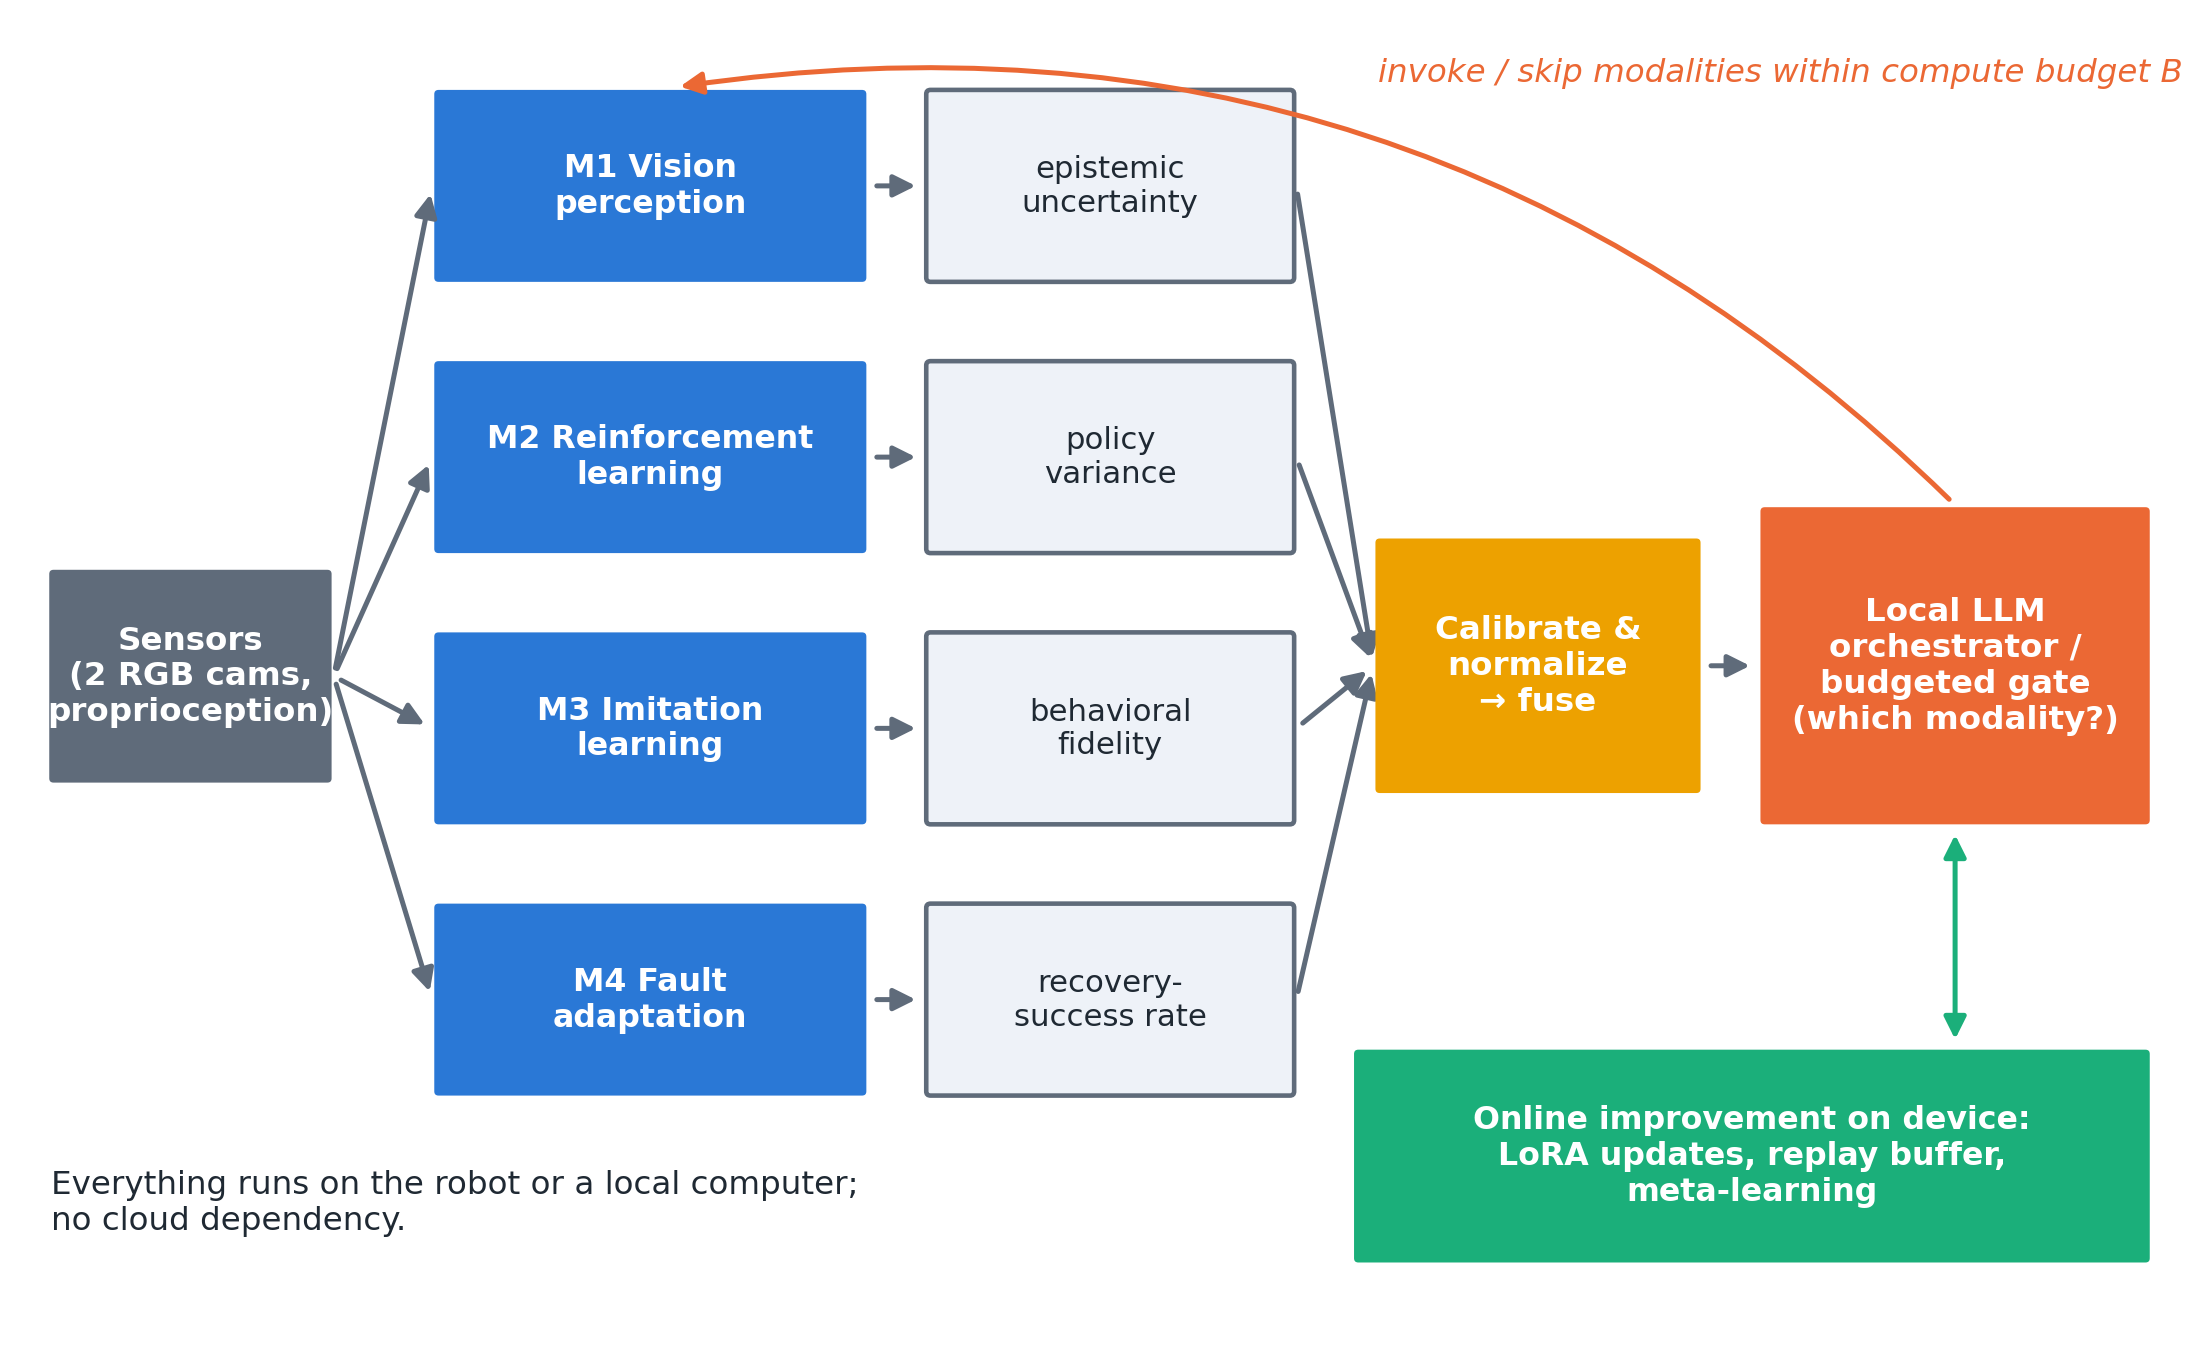
\includegraphics[width=0.85\textwidth]{figures/Fig1_architecture.png}
\caption{Architecture used to organize this survey. Four learning modalities each emit a confidence signal; signals are calibrated, normalized, and fused; a local LLM orchestrator or learned gate decides which modalities to invoke within a compute budget; and the orchestrator improves online through low-rank adaptation (LoRA) updates, replay, and meta-learning.}\label{fig:arch}
\end{figure*}


\subsection{Scope}\label{sec:scope}
We restrict attention to a single robot. We treat ``on-device'' as covering computation on the robot and on a local computer connected to it, but never a remote cloud service. This distinction matters in practice: the standard configuration of the LeKiwi mobile manipulator runs a Raspberry Pi 5 on the robot and streams observations over ZeroMQ to a laptop, where heavier policies run~\cite{Cadene2026}. Multi-robot federated learning is discussed only as a source of fusion ideas (Section \ref{sec:federated}), and quantum and neuromorphic hardware are out of scope.


\subsection{Related Surveys and Contributions}\label{sec:related}
Existing surveys cover the components of this problem separately: uncertainty in deep networks~\cite{Gawlikowski2023}, meta-learning~\cite{Hospedales2022}, continual learning~\cite{DeLange2022}, multimodal learning~\cite{Baltrusaitis2019}, federated learning~\cite{Kairouz2021,Qi2021}, imitation learning~\cite{Osa2018}, safe learning in robotics~\cite{Brunke2022,Garcia2015}, fault detection in robots~\cite{Khalastchi2018}, anomaly detection~\cite{Pang2021}, and efficient VLA models~\cite{Yu2025}. None of them addresses how heterogeneous learners should be orchestrated on resource-constrained hardware. This survey makes six contributions.

\begin{itemize}
\item A modality-by-signal taxonomy that pairs each learning modality with a confidence signal that it can emit cheaply (Table \ref{tab:signals}).
\item A graded review of 180 works, each classified by evidence level and by compute footprint relative to a Raspberry-Pi-class robot (Table \ref{tab:levels}, Fig. \ref{fig:evidence}).
\item A gap analysis showing that learned, uncertainty-aware, budget-constrained arbitration between heterogeneous learners on edge hardware has not been demonstrated (Sections \ref{sec:gap} and \ref{sec:position}, Fig. \ref{fig:position}).
\item A formal problem statement as budget-constrained, confidence-driven routing (Section \ref{sec:formal}).
\item An illustrative simulation of the effect of miscalibration on routing (Section \ref{sec:gate}).
\item An evaluation protocol for real-robot studies and a set of open challenges (Sections \ref{sec:platforms}--\ref{sec:challenges}).
\end{itemize}


\subsection{Organization}\label{sec:organization}
Section \ref{sec:method} describes the review methodology. Section \ref{sec:background} introduces the four learning modalities. Sections \ref{sec:llm} and \ref{sec:vla} review LLM orchestrators and VLA models. Sections \ref{sec:vision}--\ref{sec:fault} review the four modalities and their confidence signals. Sections \ref{sec:meta}--\ref{sec:ondevice} cover meta-learning, uncertainty fusion, and on-device adaptation, and Section \ref{sec:routing} covers adaptive computation, mixture of experts, and the formal problem statement. Section \ref{sec:platforms} discusses low-cost platforms and evaluation, Section \ref{sec:challenges} the open challenges, and Section \ref{sec:conclusion} concludes.


\section{Review Methodology}\label{sec:method}
The corpus combines a curated list of 108 works with 72 works found by structured searches of arXiv, conference proceedings (CoRL, RSS, ICRA, IROS, NeurIPS, ICML, ICLR) and publisher sites. The searches, conducted in September 2026, covered: uncertainty-aware LLM and VLA planning; efficient and edge VLAs; budget-aware model routing; RL fine-tuning of large policies; failure detection and recovery with foundation models; uncertainty fusion and calibration; continual and on-device learning; safe learning; and low-cost hardware and evaluation methodology. Every work was checked against its arXiv or publisher record, and about twenty entries of the original list needed corrections to year, venue, or authors. Each work was read from its abstract or full text and classified by evidence level (Table \ref{tab:levels}) and by compute footprint. \fillin{search strings and hit counts per source} Fig. \ref{fig:evidence} shows the distribution of evidence levels by section; 81 works are at E3, 56 at E4 and 9 at E5, and none reaches E6.

\begin{table*}[!t]
\centering
\caption{Evidence Levels Used to Classify the Reviewed Works, With the Number of Works at Each Level (n = 180)}\label{tab:levels}%
\footnotesize
\begin{tabular}{@{}>{\raggedright\arraybackslash}p{0.100\dimexpr\textwidth-10\tabcolsep\relax}>{\raggedright\arraybackslash}p{0.170\dimexpr\textwidth-10\tabcolsep\relax}>{\raggedright\arraybackslash}p{0.330\dimexpr\textwidth-10\tabcolsep\relax}>{\raggedright\arraybackslash}p{0.300\dimexpr\textwidth-10\tabcolsep\relax}>{\raggedright\arraybackslash}p{0.100\dimexpr\textwidth-10\tabcolsep\relax}@{}}
\toprule
\textbf{Level} & \textbf{Label} & \textbf{Definition} & \textbf{Example} & \textbf{n} \\ \midrule
E1 & Conceptual & Position or proposal without an algorithm or experiments & -- & 0 \\
E2 & Algorithmic or analytic & Algorithm or theory with analytic or toy evaluation & MC dropout~\cite{Gal2016}; shielding~\cite{Alshiekh2018} & 15 \\
E3 & Simulation or benchmark & Evaluated in simulation or on standard datasets & LIBERO~\cite{Liu2023b}; RouteLLM~\cite{Ong2025} & 81 \\
E4 & Real robot (laboratory) & Demonstrated on physical robots in the laboratory & Sentinel~\cite{Agia2024}; MoE-Loco~\cite{Huang2025} & 56 \\
E5 & Real robot (extensive) & Extensive real-robot evaluation or multiple platforms & OpenVLA~\cite{Kim2024}; QT-Opt~\cite{Kalashnikov2018} & 9 \\
E6 & Deployment & Sustained deployment with real users & None found & 0 \\
R/S & Review or software & Surveys, tutorials, libraries, and benchmarks & LeRobot~\cite{Cadene2026} & 19 \\
\bottomrule
\end{tabular}
\end{table*}

\begin{figure*}[!t]
\centering
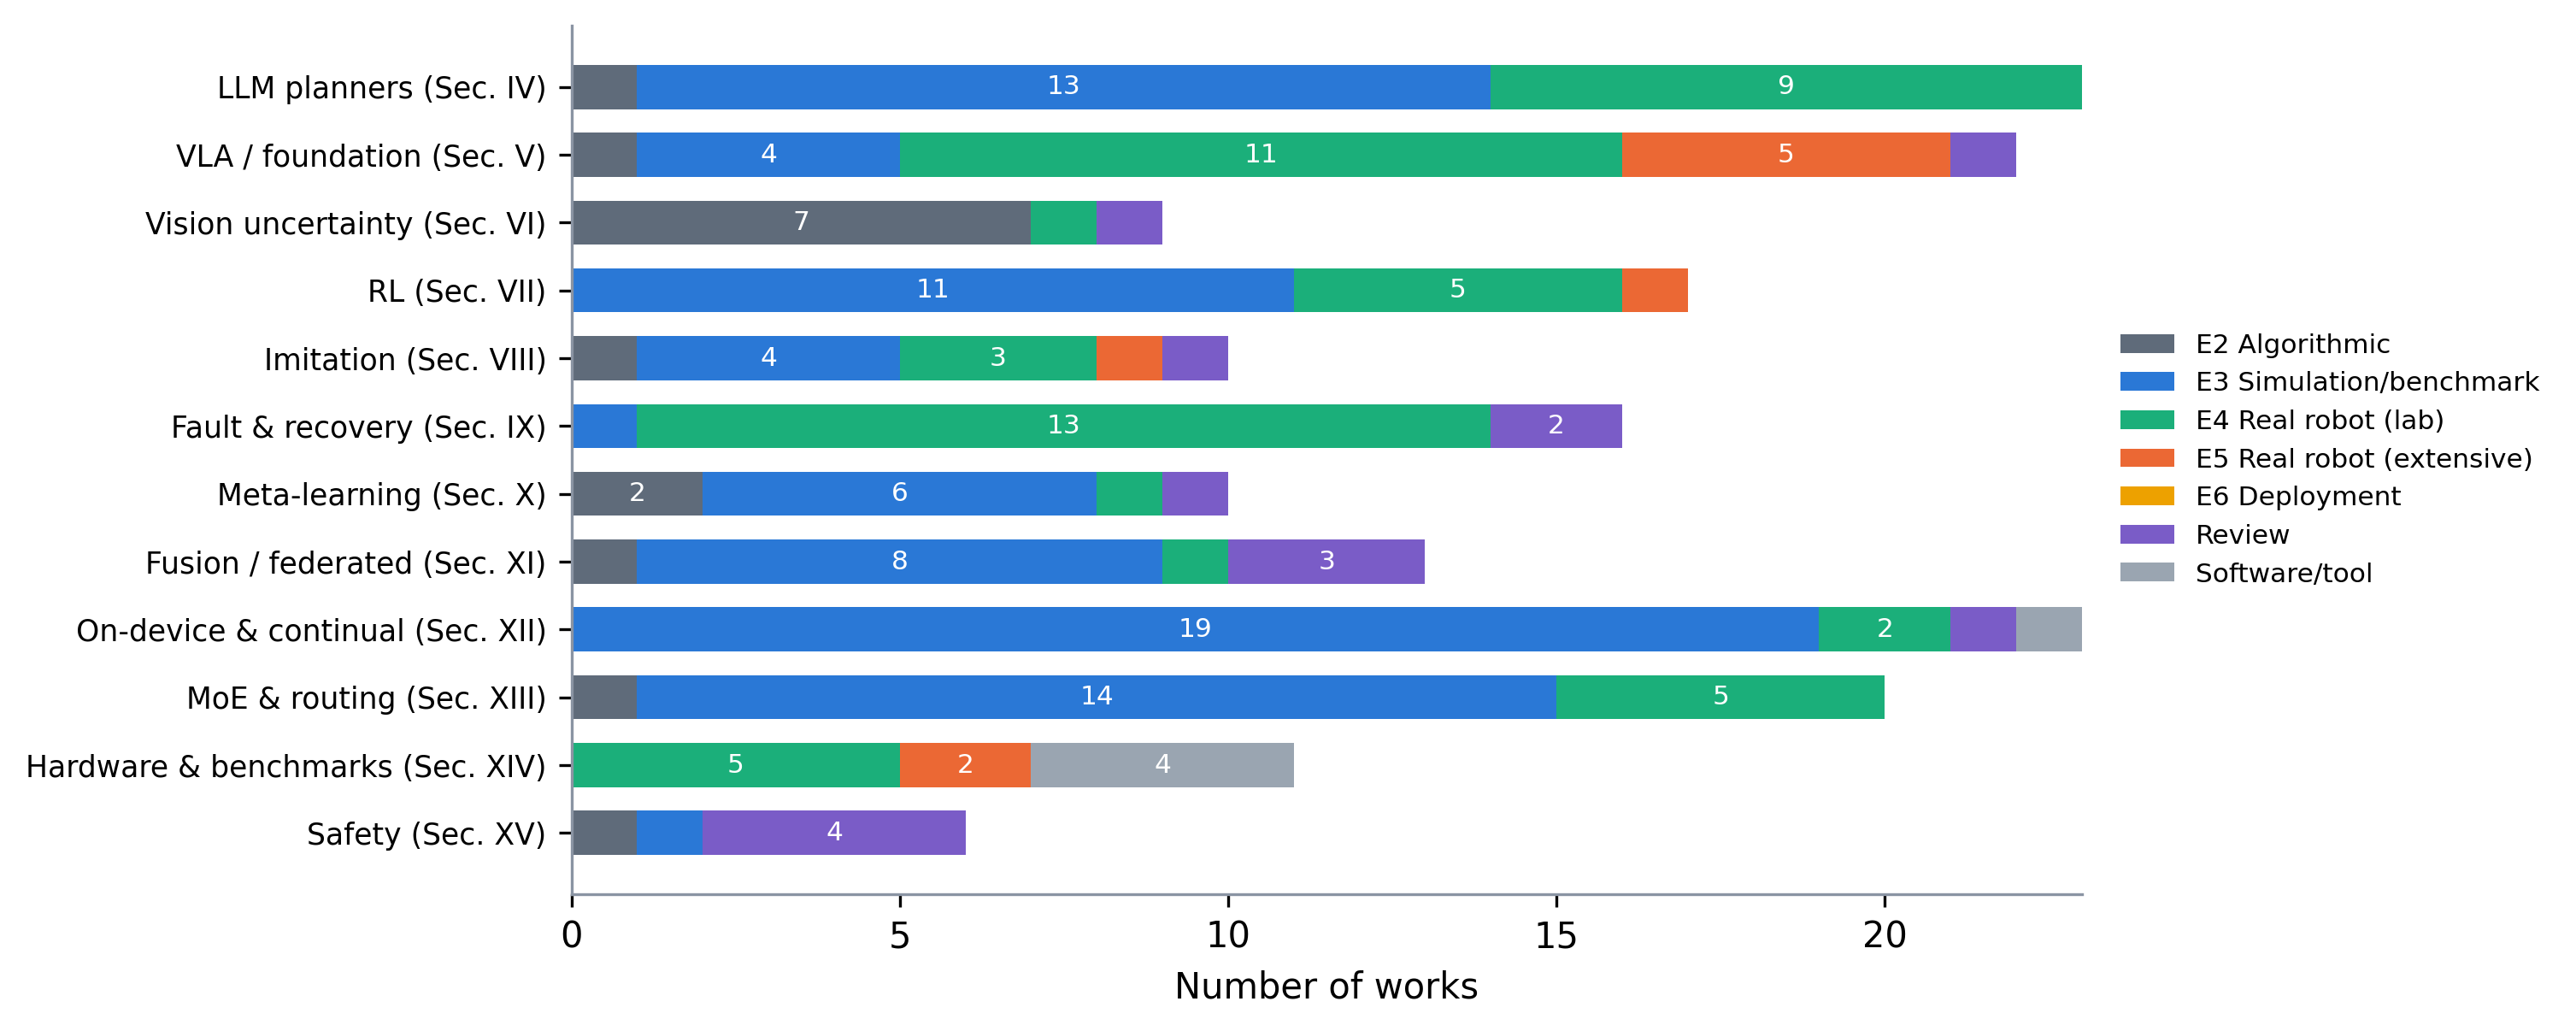
\includegraphics[width=0.85\textwidth]{figures/Fig2_evidence.png}
\caption{Evidence levels of the 180 works by survey section. E1 conceptual; E2 algorithmic or analytic; E3 simulation or benchmark; E4 real robot (laboratory); E5 real robot (extensive or multi-platform); E6 deployment. No work reaches E6.}\label{fig:evidence}
\end{figure*}

\textit{Threats to validity.} Several threats apply. The field moves quickly, and many relevant works are preprints that have not yet been peer-reviewed. Some works were classified from their abstracts rather than their full texts, which may have led to errors in the assigned evidence level; when in doubt, we assigned the lower level. The evidence levels grade how far a work goes toward a deployed robot, not its scientific quality. The compute-footprint assessment relies on figures reported in the papers, which are not measured on a common platform.


\section{Learning Modalities in Robotics}\label{sec:background}

\subsection{Overview of the Four Modalities}\label{sec:modalities}
\textit{Perception.} Perception maps camera images and other sensor readings to object identities, poses and scene structure. Foundation vision--language encoders such as CLIP provide open-vocabulary recognition~\cite{Radford2021} and underpin language-conditioned manipulation~\cite{Shridhar2021}. For an orchestrator, the key property of a perception module is whether it knows when it does not know. Bayesian approximations, ensembles and evidential outputs provide this (Section \ref{sec:vision})~\cite{Gal2016,Lakshminarayanan2017,Sensoy2018}, and uncertainty surveys map the design space~\cite{Gawlikowski2023}.

\textit{Reinforcement learning.} Deep RL learns control from reward, from value-based methods with experience replay~\cite{Mnih2015} to policy-gradient~\cite{Schulman2017} and maximum-entropy actor--critic methods~\cite{Haarnoja2018,Fujimoto2018}. Real-robot RL has reached 96\% grasp success on unseen objects, but only with large-scale data collection~\cite{Kalashnikov2018}. Model-based RL improves sample efficiency across more than 150 tasks~\cite{Hafner2023}. RL is the modality that can improve beyond its data, but it is the most expensive to run on hardware.

\textit{Imitation learning.} Imitation learning copies expert behavior~\cite{Osa2018}. Its classical difficulty is compounding error under distribution shift, which DAgger addresses with interactive data aggregation~\cite{Ross2011}. Modern imitation, using diffusion policies~\cite{Chi2023}, action-chunking transformers on low-cost hardware~\cite{Zhao2023} and implicit energy-based models~\cite{Florence2021}, learns dexterous skills from minutes of demonstrations. ACT reached 80--90\% success on six tasks with ten minutes of demonstrations~\cite{Zhao2023}.

\textit{Fault adaptation and recovery.} Robots that recover from damage use self-models~\cite{Bongard2006}, precomputed behavior repertoires searched by Bayesian optimization~\cite{Cully2015}, meta-learned dynamics models that adapt online~\cite{Nagabandi2019}, or adaptation modules trained in simulation that adjust within fractions of a second~\cite{Kumar2021}. Detecting that something has gone wrong is itself a learning problem~\cite{Pang2021,Khalastchi2018}, now addressed with foundation models (Section \ref{sec:fault}).


\subsection{Why Each Modality Alone Is Insufficient}\label{sec:insufficient}
Each modality has a characteriztic failure. Perception is brittle out of distribution and often overconfident~\cite{Guo2017,Hendrycks2017}. RL is sample-hungry and unsafe to explore on hardware~\cite{Brunke2022}. Imitation cannot exceed its demonstrations and degrades under distribution shift~\cite{Ross2011}. Fault adaptation methods are specialized to a platform or a class of damage~\cite{Kumar2021}. Robustness baked in offline, for example by domain randomization~\cite{Tobin2017}, cannot anticipate every failure. No single modality covers the situations a long-lived robot will meet.


\subsection{The Case for Composition}\label{sec:composition}
The strengths are complementary. Imitation gives fast competence, RL gives improvement~\cite{Yuan2025,Ankile2025}, perception grounds both, and fault adaptation keeps the robot operational. Several lines of work already combine two modalities. Residual RL refines imitation policies~\cite{Yuan2025,Ankile2025}, RL in the latent noise space steers diffusion policies~\cite{Wagenmaker2025}, and interactive imitation switches control between robot and human under a budget~\cite{Hoque2021}. What these combinations lack is a general, learned arbiter across more than two modalities that uses each modality's own estimate of its reliability. That arbiter is the subject of Sections \ref{sec:meta}--\ref{sec:routing}. Table \ref{tab:signals} pairs each modality with the confidence signal it can emit and the cost of computing it.

\begin{table*}[!t]
\centering
\caption{The Four Learning Modalities and Their Confidence Signals}\label{tab:signals}%
\footnotesize
\begin{tabular}{@{}>{\raggedright\arraybackslash}p{0.160\dimexpr\textwidth-10\tabcolsep\relax}>{\raggedright\arraybackslash}p{0.160\dimexpr\textwidth-10\tabcolsep\relax}>{\raggedright\arraybackslash}p{0.280\dimexpr\textwidth-10\tabcolsep\relax}>{\raggedright\arraybackslash}p{0.180\dimexpr\textwidth-10\tabcolsep\relax}>{\raggedright\arraybackslash}p{0.220\dimexpr\textwidth-10\tabcolsep\relax}@{}}
\toprule
\textbf{Modality} & \textbf{Confidence signal} & \textbf{Typical estimator} & \textbf{Extra compute} & \textbf{Calibration need} \\ \midrule
M1 Vision perception & Epistemic uncertainty & MC dropout~\cite{Gal2016}, ensembles~\cite{Lakshminarayanan2017}, evidential~\cite{Sensoy2018} & None (evidential) to N\ensuremath{\times } (ensembles, MC) & Temperature scaling~\cite{Guo2017} \\
M2 Reinforcement learning & Policy variance & Entropy~\cite{Haarnoja2018}, critic or head ensembles~\cite{Osband2016}, novelty~\cite{Burda2019} & None (entropy) to K heads & High: entropy is not a success probability \\
M3 Imitation & Behavioral fidelity & Action spread~\cite{Agia2024}, density and OOD scores~\cite{Xu2025,Romer2025} & Several samples or a small density model & Temperature~\cite{Wu2024}; conformal thresholds \\
M4 Fault adaptation & Recovery-success rate & Beta posterior over outcomes; anomaly scores & Negligible & Low (counts outcomes) but slow to accumulate \\
\bottomrule
\end{tabular}
\end{table*}


\section{LLMs as Planners and Orchestrators}\label{sec:llm}

\subsection{LLM-Driven Planning and Tool Use}\label{sec:llmplan}
LLMs were first shown to produce executable plans for embodied agents zero-shot, with a trade-off between executability and correctness~\cite{Huang2022a}. SayCan grounded the choice among robot skills by multiplying LLM relevance with learned affordance values~\cite{Ahn2022}. Inner Monologue closed the loop with textual feedback on success and scene state~\cite{Huang2022b}. Code as Policies~\cite{Liang2023} and ProgPrompt~\cite{Singh2023} generated programs that call perception and control APIs. LM-Nav composed three frozen models for navigation~\cite{Shah2022}, LLM-Planner re-planned on failure with little paired data~\cite{Song2023}, VoxPoser composed 3D value maps~\cite{Huang2023a}, and Language to Rewards let an LLM specify rewards for model-predictive control, solving 90\% of tasks against 50\% for a primitive-skill baseline~\cite{Yu2023}. Plan-Seq-Learn used an LLM for high-level plans and RL for low-level skills~\cite{Dalal2024}. PaLM-E injected continuous observations into a 562-billion-parameter model~\cite{Driess2023}, and Voyager built a growing skill library in Minecraft~\cite{Wang2024a}. These systems establish that an LLM can decide which module to call. However, they rely on large cloud models and do not learn the calling policy from robot experience.


\subsection{Agent Loops and Tool Calling}\label{sec:agents}
ReAct interleaves reasoning and acting, improving success by 34 and 10 percentage points on ALFWorld and WebShop over imitation and RL baselines~\cite{Yao2023a}. Toolformer teaches a model, by self-supervision, when to call which tool~\cite{Schick2023}. This is the closest analog to learning when to invoke each modality, although it is offline and not embodied. Reflexion improves through verbal reflection stored in memory, without weight updates~\cite{Shinn2023}, and Tree of Thoughts searches over reasoning paths at much higher inference cost~\cite{Yao2023b}. A second generation updates weights. FireAct fine-tuned a 7B model on agent trajectories~\cite{Chen2023b}, AgentTuning instruction-tuned open models on agent data~\cite{Zeng2024}, Retroformer trained a small reflection model by policy gradient~\cite{Yao2024}, and RL fine-tuning of vision--language models as decision agents outperformed GPT-4V on several tasks~\cite{Zhai2024}. These results show that small orchestrators can be improved by fine-tuning, a prerequisite for learned orchestration.


\subsection{Limits of a Frozen LLM Orchestrator}\label{sec:frozen}
A frozen LLM orchestrator has three weaknesses in the edge setting. It does not know when it is wrong. KnowNo addressed this with conformal prediction, asking for help when the prediction set over plan options contains more than one element and providing statistical guarantees on task completion~\cite{Ren2023}. Introspective planning tightened these bounds~\cite{Liang2024}, and the approach extends to multi-robot planning~\cite{Wang2024c} and to deciding when to stop exploring~\cite{Ren2024}. A frozen LLM also cannot adapt its calling policy to the particular robot, whose modules succeed or fail in ways no pretraining corpus describes. Finally, its cost is fixed: it cannot decide to think less when the situation is easy. Recent work learns exactly this with an RL meta-policy that decides when to invoke expensive LLM reasoning. That meta-policy cut LLM inference time by more than 60\% with a small loss in success~\cite{Liu2026}.


\subsection{Learned Versus Hard-Coded Orchestration}\label{sec:gap}
Table \ref{tab:orch} summarizes the orchestration literature along four axes. The axes are whether the orchestrator is learned, whether it uses calibrated uncertainty, whether it respects a compute budget, and whether it runs on edge hardware. Existing systems satisfy at most two. The closest are policy steering that decides whether to act, ask or request intervention~\cite{Yuan2026}; fast--slow anomaly handling with small language models~\cite{Sinha2024}; budget-aware reasoning~\cite{Liu2026}; and budgeted human--robot gating~\cite{Hoque2021}. None of them arbitrates between heterogeneous learning modalities, and none learns the arbitration online on the robot. This is the gap targeted by the framework of this survey.

\begin{table*}[!t]
\centering
\caption{Orchestration Approaches Against Four Requirements of Learned Edge Orchestration}\label{tab:orch}%
\footnotesize
\begin{tabular}{@{}>{\raggedright\arraybackslash}p{0.320\dimexpr\textwidth-10\tabcolsep\relax}>{\raggedright\arraybackslash}p{0.170\dimexpr\textwidth-10\tabcolsep\relax}>{\raggedright\arraybackslash}p{0.170\dimexpr\textwidth-10\tabcolsep\relax}>{\raggedright\arraybackslash}p{0.150\dimexpr\textwidth-10\tabcolsep\relax}>{\raggedright\arraybackslash}p{0.190\dimexpr\textwidth-10\tabcolsep\relax}@{}}
\toprule
\textbf{Approach} & \textbf{Learned policy?} & \textbf{Calibrated uncertainty?} & \textbf{Compute budget?} & \textbf{Edge-deployable?} \\ \midrule
SayCan, Inner Monologue~\cite{Ahn2022,Huang2022b} & No (frozen LLM) & No & No & No (cloud LLM) \\
Code as Policies, ProgPrompt~\cite{Liang2023,Singh2023} & No & No & No & Generated code yes; LLM no \\
ReAct, Reflexion~\cite{Yao2023a,Shinn2023} & In-context only & No & No & Depends on LLM \\
Toolformer~\cite{Schick2023} & Yes (offline) & No & No & Mid-size model \\
FireAct, Retroformer~\cite{Chen2023b,Yao2024} & Yes (fine-tuned) & No & No & Possibly (small models) \\
KnowNo, introspective planning~\cite{Ren2023,Liang2024} & No & Yes (conformal) & No & Calibration yes; LLM no \\
Act, ask, or learn~\cite{Yuan2026} & Partly (residual learning) & Yes (conformal) & No & No (large VLM) \\
Fast/slow anomaly handling~\cite{Sinha2024} & Classifier trained & Partly & Implicitly (fast path) & Fast path plausibly \\
RouteLLM, Hybrid LLM, AutoMix~\cite{Ong2025,Ding2024,Aggarwal2024} & Yes & Partly (predicted quality) & Yes & Router yes \\
RARRL~\cite{Liu2026} & Yes (RL) & No & Yes & Not stated \\
ThriftyDAgger~\cite{Hoque2021} & Thresholds & Novelty and risk & Yes (human budget) & Yes \\
Target (unoccupied) & Yes, online on device & Yes, across four modalities & Yes & Yes \\
\bottomrule
\end{tabular}
\end{table*}


\section{VLA and Robot Foundation Models}\label{sec:vla}

\subsection{Vision--Language--Action Models}\label{sec:vlamodels}
VLA models map images and language directly to actions. RT-1 trained a transformer on large real-robot datasets~\cite{Brohan2023a}, and RT-2 co-fine-tuned a vision--language model to transfer web knowledge to control, evaluated over 6,000 trials~\cite{Brohan2023b}. OpenVLA, a 7B open model, outperformed the 55B RT-2-X by 16.5 percentage points in absolute success and can be fine-tuned with LoRA on consumer GPUs~\cite{Kim2024}. Octo~\cite{Octo2024}, \ensuremath{\pi}0~\cite{Black2024}, RoboCat~\cite{Bousmalis2023}, Gato~\cite{Reed2022}, VIMA~\cite{Jiang2023}, PerAct~\cite{Shridhar2022} and RoboFlamingo~\cite{Li2024a} extend the generalizt program, and cross-embodiment datasets support it~\cite{OXE2024}.


\subsection{Limitations of Generalizt Policies on Edge Hardware}\label{sec:generalizt}
Generalizt policies are monolithic. They offer no handle for allocating computation across sub-skills, no native uncertainty estimate, and no mechanism for on-device improvement beyond offline fine-tuning. RL fine-tuning methods address the last point, for example raising OpenVLA's real-world success from 40\% to 70\% in 40 minutes~\cite{Mark2025}, reaching 96.3\% average success after 45--90 minutes of online training~\cite{Chen2025}, and scaling RL for VLAs~\cite{Lu2025,Li2026}. All of these need GPUs.


\subsection{Memory, Latency, and Compute}\label{sec:memory}
Fig. \ref{fig:size} compares model sizes with the memory of a 4 GB Raspberry Pi 5. Storing the weights of a 2-billion-parameter model in 16-bit precision alone would fill that memory. OpenVLA (7B) and larger models therefore require an off-board GPU. The LeRobot paper reports that ACT needs about 5 ms and 211 MB per inference on an RTX 4090, against about 209 ms and 13.3 GB for \ensuremath{\pi}0~\cite{Cadene2026}. Efficiency work narrows the gap: SmolVLA performs comparably to VLAs about ten times larger and runs on consumer GPUs or CPUs~\cite{Shukor2025}; TinyVLA~\cite{Wen2025} and EdgeVLA~\cite{Budzianowski2025} target fast inference; OpenVLA-OFT achieved 26 times higher throughput~\cite{Kim2025}; FAST compresses action tokens~\cite{Pertsch2025}; 1-bit and post-training quantization cut memory by up to 11 times~\cite{Wang2025a,Zhang2026a}; and state-space backbones reduce latency~\cite{Liu2024a}. A survey maps efficient VLA design~\cite{Yu2025}. Even so, only the smallest policies are plausible on the Pi itself.

\begin{figure}[!t]
\centering
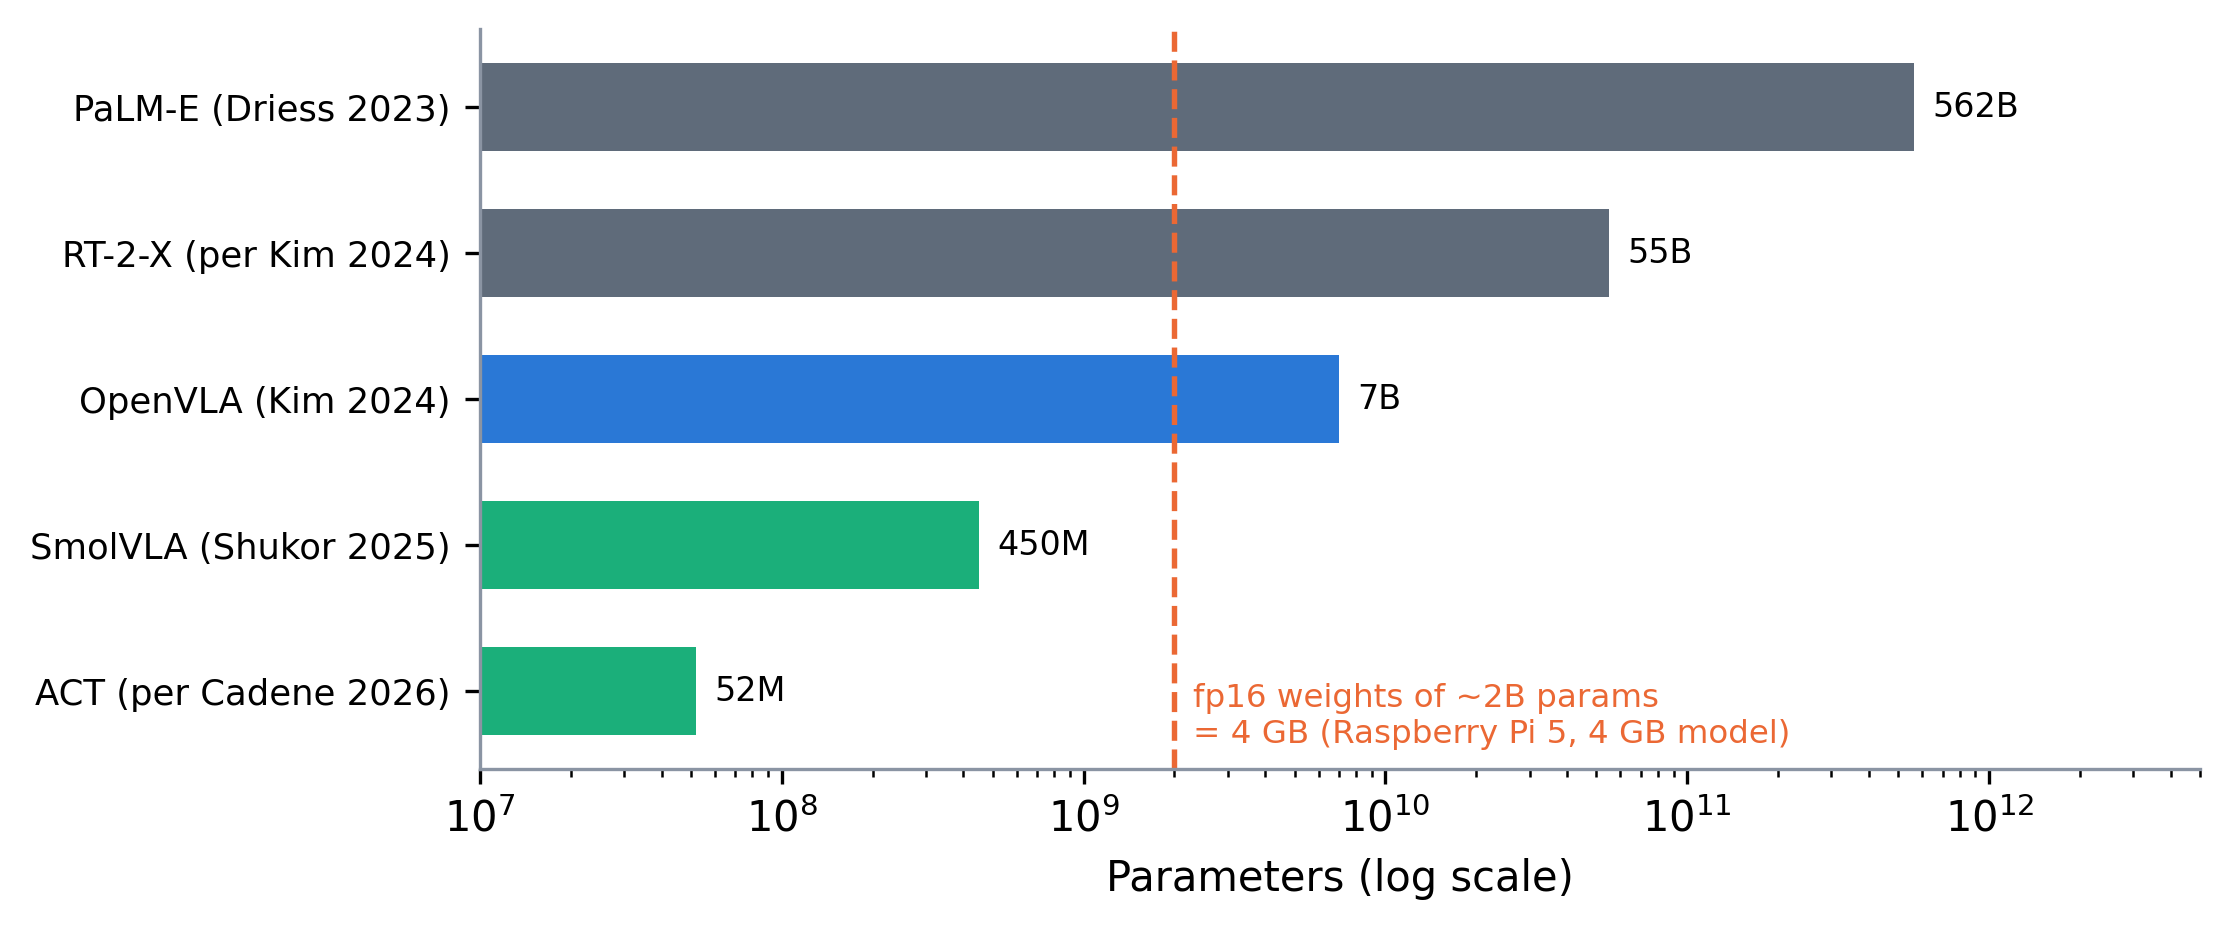
\includegraphics[width=\columnwidth]{figures/Fig3_model_size.png}
\caption{Parameter counts of representative planners and policies (log scale) compared with a 4 GB Raspberry Pi 5, whose memory holds the 16-bit weights of at most about 2 billion parameters before any activations or operating system. Sizes from the cited papers; ACT's size as reported in the LeRobot paper.}\label{fig:size}
\end{figure}


\subsection{Modular Policies With a Small Local Orchestrator}\label{sec:modular}
The evidence favors a modular design: small specialized policies (ACT-scale imitation, compact RL policies, lightweight perception) plus a small orchestrator. Distilling planning ability into a 3B on-device model recovered over 93\% of GPT-4o's performance~\cite{Ravichandran2025}, and small routers can decide when larger models are needed (Section \ref{sec:routing}). The trade-off is that the robot loses the broad generalization of large VLAs. Whether orchestration recovers enough adaptivity to compensate is an open empirical question.


\section{Vision Perception With Epistemic Uncertainty}\label{sec:vision}

\subsection{Perception Pipeline}\label{sec:pipeline}
The perception modality turns camera images into task-relevant state such as object classes, masks and poses. On a low-cost robot with two RGB cameras and no depth sensor, 2D detection and segmentation with language-conditioned encoders~\cite{Radford2021,Shridhar2021} are the realiztic options. Voxel-based methods such as PerAct assume depth input~\cite{Shridhar2022}. Domain randomization yields detectors robust enough for 1.5 cm localization in clutter~\cite{Tobin2017}.


\subsection{Epistemic Uncertainty Quantification}\label{sec:uq}
Epistemic uncertainty reflects what the model does not know and should shrink with more data, whereas aleatoric uncertainty reflects inherent noise~\cite{Kendall2017}. Only epistemic uncertainty tells an orchestrator that another modality, or more data, could help.

\textit{Monte Carlo dropout.} Keeping dropout active at test time and averaging several stochastic passes approximates Bayesian inference~\cite{Gal2016}. It needs no retraining, but its cost grows linearly with the number of passes, and the quality of its uncertainty is debated.

\textit{Ensembles.} Deep ensembles give well-calibrated uncertainty, as good as or better than approximate Bayesian networks, and higher uncertainty on out-of-distribution inputs~\cite{Lakshminarayanan2017}. Their cost scales with the number of members, which is the central edge trade-off. Shared-backbone ensembles (multiple heads) reduce the cost, as bootstrapped DQN does in RL~\cite{Osband2016}.

\textit{Evidential deep learning.} Evidential networks output the parameters of a distribution over predictions in a single pass: a Dirichlet for classification~\cite{Sensoy2018} or a normal-inverse-gamma for regression~\cite{Amini2020}. This makes them the cheapest source of epistemic confidence and therefore attractive for a Raspberry Pi. Their calibration can degrade out of distribution. The simplest out-of-distribution signal, the maximum softmax probability, costs nothing extra but is often overconfident~\cite{Hendrycks2017}.


\subsection{Calibration}\label{sec:calibration}
Modern networks are systematically overconfident, and a single temperature parameter fitted on held-out data corrects much of this~\cite{Guo2017}. For VLAs, confidence predicts task success poorly without correction; prompt ensembles and Platt scaling improve it~\cite{Zollo2025}. Calibration is a prerequisite for orchestration: a gate that compares confidences across modalities is only as good as their calibration (Section \ref{sec:comparable}).


\subsection{Cost Versus Uncertainty Quality on Edge Hardware}\label{sec:uqcost}
Table \ref{tab:uqcost} compares the options. Temperature scaling and evidential outputs are essentially free, MC dropout and ensembles multiply inference, and conformal methods add a cheap calibration step on top of any score~\cite{Ren2023}. For a Pi-class robot, a practical design is an evidential or temperature-scaled detector, with ensembles reserved for offline calibration.

\begin{table*}[!t]
\centering
\caption{Uncertainty Estimators: Cost and Suitability for a Raspberry-Pi-Class Robot}\label{tab:uqcost}%
\footnotesize
\begin{tabular}{@{}>{\raggedright\arraybackslash}p{0.270\dimexpr\textwidth-8\tabcolsep\relax}>{\raggedright\arraybackslash}p{0.200\dimexpr\textwidth-8\tabcolsep\relax}>{\raggedright\arraybackslash}p{0.250\dimexpr\textwidth-8\tabcolsep\relax}>{\raggedright\arraybackslash}p{0.280\dimexpr\textwidth-8\tabcolsep\relax}@{}}
\toprule
\textbf{Method} & \textbf{Inference cost} & \textbf{Strength} & \textbf{Weakness} \\ \midrule
Max softmax~\cite{Hendrycks2017} & 1 pass & Free & Overconfident \\
Temperature scaling~\cite{Guo2017} & 1 pass + scalar & Fixes global miscalibration & Needs held-out data; not per-input epistemic \\
Evidential~\cite{Sensoy2018,Amini2020} & 1 pass & Epistemic signal in one pass & Can be miscalibrated out of distribution \\
MC dropout~\cite{Gal2016} & T passes & No retraining & Latency; quality debated \\
Deep ensembles~\cite{Lakshminarayanan2017} & M models & Strong, well calibrated & M\ensuremath{\times } memory and compute \\
Conformal prediction~\cite{Ren2023} & Negligible over base score & Distribution-free coverage & Assumes exchangeability \\
\bottomrule
\end{tabular}
\end{table*}


\section{Reinforcement Learning With Policy Variance}\label{sec:rl}

\subsection{RL Backbones}\label{sec:rlback}
\textit{Policy-gradient methods.} Proximal policy optimization (PPO) is the default on-policy algorithm, balancing sample complexity, simplicity and wall-clock time~\cite{Schulman2017}. Its small policy and value networks run comfortably on a Raspberry Pi, but training is usually done in simulation on a workstation.

\textit{Value-based and off-policy methods.} DQN introduced experience replay for deep RL~\cite{Mnih2015}. Off-policy actor--critic methods such as SAC~\cite{Haarnoja2018} and TD3~\cite{Fujimoto2018} are more sample-efficient for continuous control. Hindsight experience replay makes sparse-reward robot tasks learnable by relabeling goals, and its simulated policies transferred to a physical robot~\cite{Andrychowicz2017}. Offline RL learns from fixed buffers without new interaction; conservative Q-learning often achieved two to five times higher final return than earlier offline methods~\cite{Kumar2020}. This is relevant to learning from on-device logs. Model-based RL with world models improves sample efficiency~\cite{Hafner2023}, but its memory cost is high for edge training.


\subsection{Policy and Value Variance as Confidence Signals}\label{sec:rlconf}
An RL policy's confidence can be read in two ways: from the spread of its action distribution, or from disagreement among value estimates.

\textit{Policy entropy.} Maximum-entropy RL makes the policy stochastic by design, so its entropy is available at no extra cost~\cite{Haarnoja2018}. Entropy, however, mixes aleatoric choice (several good actions) with epistemic ignorance (unknown state), and it is not calibrated to success probability. Calibration against observed outcomes is therefore needed before entropy is compared with other modalities' signals (Section \ref{sec:comparable}).

\textit{Ensembles and twin critics.} Bootstrapped DQN uses multiple heads on a shared network to approximate a posterior and drive deep exploration, improving learning times across most Atari games~\cite{Osband2016}. Head disagreement is a direct epistemic signal. TD3's twin critics reduce overestimation but do not quantify uncertainty~\cite{Fujimoto2018}. Random network distillation provides a cheap novelty score for states the agent has not visited~\cite{Burda2019}, which could also trigger the fault modality. For the orchestrator, a small ensemble of critics or a novelty score is a practical policy-variance signal.


\subsection{Sample Efficiency on Edge Hardware}\label{sec:rledge}
Training RL on the robot is limited by sample efficiency and safety. Three strategies reduce the burden. The first is refining an imitation policy with a small residual RL policy~\cite{Yuan2025,Ankile2025}. The second is running RL in the latent noise space of a diffusion policy without changing its weights, which achieved sample-efficient real-world improvement~\cite{Wagenmaker2025}. The third is fine-tuning large policies with offline-to-online RL~\cite{Mark2025,Chen2025,Lu2025,Li2026}, which needs a GPU. On a Pi-class robot, only the first two are realiztic on board; heavier updates must run asynchronously on a local computer (Section \ref{sec:feasibility}).


\section{Imitation Learning With Behavioral Fidelity}\label{sec:il}

\subsection{Learning From Demonstration}\label{sec:lfd}
\textit{Behavioral cloning.} Behavioral cloning (BC) regresses actions on observations. Its compounding-error problem motivated DAgger, which provides no-regret guarantees by aggregating expert labels on the learner's own state distribution~\cite{Ross2011}. Modern BC is expressive. Diffusion policies model multimodal action distributions and improved on prior methods by 46.9\% on average~\cite{Chi2023}. ACT predicts action chunks on low-cost bimanual hardware~\cite{Zhao2023}. Implicit BC handles discontinuous actions with energy-based models~\cite{Florence2021}. Language-conditioned BC generalized to 24 unseen tasks with 44\% average success~\cite{Jang2021}, and learning from unstructured play covered about four times more interaction space than demonstrations~\cite{Lynch2019}. Best practice for learning from offline human demonstrations is documented in robomimic~\cite{Mandlekar2021}.

\textit{Inverse reinforcement learning.} Adversarial imitation matches the expert's state--action occupancy rather than its actions~\cite{Ho2016}. It is more robust to distribution shift in principle, but its adversarial training is unstable and sample-hungry on real robots.

\textit{Multimodal imitation.} Action multimodality, where several distinct actions are correct, is handled by diffusion~\cite{Chi2023} and energy-based models~\cite{Florence2021}. Multimodal inputs such as language and vision are handled by VLAs and multimodal prompts~\cite{Jiang2023}.


\subsection{Behavioral Fidelity as Confidence}\label{sec:fidelity}
Behavioral fidelity is the degree to which the policy is operating within the distribution of its demonstrations, where its actions are reliable.

\textit{Action-distribution spread.} For generative policies, the spread of sampled actions is a natural signal. Runtime monitors use the temporal consistency of sampled action chunks~\cite{Agia2024} and action-chunk entropy~\cite{Romer2025} to detect erratic failures. Per-task temperature scaling of language-conditioned imitation policies improved success without retraining, for example from 79.6\% to 97.1\% on block stacking with distractors~\cite{Wu2024}. A caveat is that the spread of a diffusion policy reflects both genuine multimodality and uncertainty, so it must be calibrated against outcomes.

\textit{Density and reconstruction scores.} A second signal is how well the current observation can be reconstructed or density-estimated from demonstration data. FAIL-Detect learns such scores from successful demonstrations only and sets thresholds by conformal prediction; its flow-based density signal was the most consistently effective~\cite{Xu2025}. FIPER combines observation-space out-of-distribution scores with action entropy~\cite{Romer2025}. These are practical fidelity signals because they need no failure data.


\subsection{Fast Adaptation From Few Demonstrations}\label{sec:fewshot}
One-shot imitation meta-learns to imitate from a single demonstration~\cite{Duan2017}. ACT learns from about ten minutes of demonstrations~\cite{Zhao2023}, and Mobile ALOHA's co-training raised success by up to 90\% with 50 demonstrations per task~\cite{Fu2024}. Meta-learned adapters improved forward transfer over LoRA and raised real-robot success from 60\% to 84\% with 20 demonstrations~\cite{Zhu2025}. Few-shot imitation is therefore the modality through which the orchestrator can acquire new behaviors fastest.


\section{Fault Adaptation and Recovery}\label{sec:fault}

\subsection{Fault Detection}\label{sec:faultdet}
Classical fault detection and diagnosis for robots is reviewed by Khalastchi and Kalech~\cite{Khalastchi2018}, and deep anomaly detection by Pang et al.~\cite{Pang2021}. Foundation models have transformed the area. REFLECT summarizes multisensory experience for an LLM to explain failures and plan corrections~\cite{Liu2023c}. AHA fine-tunes a VLM to detect and explain manipulation failures, beating GPT-4o by 10.3 percentage points~\cite{Duan2025}. RoboFAC improved failure-analysis accuracy by 34.1 points over GPT-4o~\cite{Ye2025}. SAFE reads a VLA's internal features to predict failure across tasks~\cite{Gu2025}. Sentinel combines a cheap consistency check with a VLM progress check and detected 18\% more failures than either alone~\cite{Agia2024}. Most relevant to edge deployment, Sinha et al. use a fast embedding-based anomaly classifier with small language models and fall back to slower generative reasoning only when needed~\cite{Sinha2024}. This fast--slow pattern mirrors budgeted orchestration.


\subsection{Online Adaptation to Damage or Malfunction}\label{sec:damage}
\textit{Resilient robots and meta-adaptation.} Continuous self-modeling let a robot infer its damaged morphology and synthesize new gaits~\cite{Bongard2006}. Intelligent trial-and-error searches a precomputed behavior map with Bayesian optimization to find compensatory behaviors within a few trials~\cite{Cully2015}. Meta-RL for dynamic environments adapts a learned dynamics model within a few steps to broken legs or new terrain~\cite{Nagabandi2019}. This is the closest prior art to combining fault adaptation with meta-learning, but it uses a single learner. RMA adapts legged locomotion in fractions of a second with a small onboard network~\cite{Kumar2021}, showing that real-time adaptation modules fit on embedded hardware.

\textit{Recovery strategies and replanning.} Recovery can mean re-invoking a different modality, asking a human, or replanning. Language corrections from a user improved a hierarchical policy without extra teleoperation~\cite{Shi2024}, and human-in-the-loop deployment learning reweights intervention data for continual improvement~\cite{Liu2023}. For the orchestrator, recovery is an action choice, and switching modality is a recovery strategy in its own right.


\subsection{Recovery-Success Rate as Confidence}\label{sec:recovery}
The fault modality's confidence is its empirical recovery-success rate for the current fault class, which can be maintained as a Beta posterior over successes and failures. Unlike the other signals, it is directly calibrated because it counts outcomes, but it is only available after enough attempts. Conformal thresholds give failure detectors false-alarm guarantees from successful data alone~\cite{Xu2025,Romer2025}.


\section{Meta-Learning and Learning to Learn}\label{sec:meta}

\subsection{Foundations}\label{sec:metafound}
MAML learns an initialization that adapts in a few gradient steps~\cite{Finn2017}, Reptile does so with first-order updates that are cheaper in memory~\cite{Nichol2018}, and prototypical networks adapt without gradients by comparing embeddings with class prototypes~\cite{Snell2017}. Learned optimizers meta-learn the update rule itself~\cite{Andrychowicz2016}. A survey organizes the field~\cite{Hospedales2022}.


\subsection{Meta-Reinforcement Learning}\label{sec:metarl}
RL\ensuremath{^2} trains a recurrent policy whose hidden state implements a learning algorithm~\cite{Duan2016}. PEARL infers a probabilistic task context and was 20--100 times more sample-efficient than earlier meta-RL~\cite{Rakelly2019}, and VariBAD maintains a belief over tasks and acts under it~\cite{Zintgraf2020}. Meta-World showed that algorithms struggle with multiple tasks even with only ten training tasks~\cite{Yu2019}, a warning for orchestrators trained on narrow task distributions.


\subsection{The Orchestrator as a Meta-Learner}\label{sec:orchmeta}
The orchestrator does not learn a task; it learns how to use learners. This places it in the meta-learning family, with two roles.

\textit{Routing.} Given fused confidences and context, the orchestrator selects which modality to call. VariBAD's belief-conditioned action selection~\cite{Zintgraf2020} and PEARL's context inference~\cite{Rakelly2019} provide the formal template: treat the unknown reliability of each modality in the current situation as a latent task variable, and route under the posterior. Routing mechanisms are reviewed in Section \ref{sec:routing}.

\textit{Fast adaptation.} When a new task or robot condition appears, the orchestrator should adapt its routing within a few episodes. Online meta-learned adapters for robot policies show this is achievable with small parameter budgets~\cite{Zhu2025}, and one-shot imitation shows the analogous result for policies~\cite{Duan2017}.


\subsection{Training the Orchestrator on Task Distributions}\label{sec:taskdist}
Meta-training requires a distribution of situations in which different modalities are best. Benchmarks such as Meta-World~\cite{Yu2019}, LIBERO~\cite{Liu2023b}, CALVIN~\cite{Mees2022} and RLBench~\cite{James2020} provide simulated task families, but none varies which learning modality is appropriate. A practical approach is to pretrain the routing policy in simulation with injected faults and perception noise, then adapt it on the robot.


\section{Uncertainty Fusion and Decentralized Confidence Signals}\label{sec:fusion}

\subsection{Heterogeneous Confidence Signals}\label{sec:hetero}
The four signals differ in scale, semantics and cost (Table \ref{tab:signals}).

\textit{Vision epistemic uncertainty.} Obtained by MC dropout, ensembles or evidential outputs, then temperature-scaled (Section \ref{sec:vision}).

\textit{RL policy variance.} Obtained from policy entropy or critic-ensemble disagreement (Section \ref{sec:rlconf}). It is unbounded and must be mapped to a probability of success.

\textit{Imitation behavioral fidelity.} Obtained from action spread, density or reconstruction scores (Section \ref{sec:fidelity}). Uncertainty for flow-based VLAs can be estimated from disagreement between velocity fields, with better calibration and at least 22\% fewer samples than baselines~\cite{Romer2026a}.

\textit{Fault recovery-success rate.} Obtained as an empirical success rate (Section \ref{sec:recovery}); it is calibrated by construction but slow to accumulate.


\subsection{Making Confidences Comparable}\label{sec:comparable}
To be compared, all signals must be expressed as calibrated estimates of the same quantity, the probability that invoking this modality now will succeed. Temperature scaling~\cite{Guo2017}, Platt scaling~\cite{Zollo2025} and conformal prediction~\cite{Ren2023,Lindemann2023,Xu2025} provide the tools, but none addresses cross-modality calibration, where signals of different origin must be placed on one scale. We know of no work that calibrates confidences from heterogeneous learners against a shared success variable on a robot; this is an open challenge (Section \ref{sec:ch-calib}). Our simulation (Section \ref{sec:gate}) illustrates the stakes: overconfident RL and imitation signals reduced routing success from 0.85 to 0.81, and a per-modality linear recalibration fitted on a separate set restored 0.85.


\subsection{Federated Learning and Decentralized Confidence Fusion}\label{sec:federated}
\textit{Federated learning versus confidence fusion.} In classic federated learning, clients train locally and a server averages weights. FedAvg reduced communication rounds by 10--100 times over synchronous SGD~\cite{McMahan2017}, and FedProx handles heterogeneous clients~\cite{Li2020}. Surveys cover the field~\cite{Kairouz2021} and its extension to RL~\cite{Qi2021}. In the orchestration setting, ``federated'' is used differently: modalities stay separate and share only confidence signals, not weights or data, with the orchestrator. To avoid confusion with FL, we recommend a precise definition such as ``decentralized confidence fusion``: each modality computes and calibrates its own signal locally, and only the scalar signals are aggregated.

\textit{Fusion methods.} Three families are available. Uncertainty-weighted averaging learns weights from each head's uncertainty, as in multi-task loss weighting~\cite{Kendall2018}. Evidential fusion combines per-source Dirichlet evidence with Dempster--Shafer rules, giving calibrated multi-view uncertainty~\cite{Han2021,Han2022a}, and dynamic fusion weights modalities by their estimated informativeness per sample~\cite{Han2022b}. Learned gating and attention treat fusion as routing (Section \ref{sec:routing}). Multimodal learning surveys supply the vocabulary~\cite{Baltrusaitis2019}. Evidential fusion is attractive for edge use because its combination rule is closed-form and cheap.


\subsection{From Fused Confidence to Allocation}\label{sec:allocation}
The fused confidence vector becomes the input to the gate (Section \ref{sec:gate}). Decisions include which modality to run, whether to run a second one for verification, and whether to ask a human. Policy steering that chooses between acting, asking and requesting intervention~\cite{Yuan2026} and conformal help-seeking~\cite{Ren2023,Liang2024} show how calibrated uncertainty can drive such discrete choices with guarantees.


\section{On-Device Adaptation: LoRA, Replay, and Continual Learning}\label{sec:ondevice}

\subsection{Parameter-Efficient Adaptation}\label{sec:peft}
\textit{Low-rank adaptation.} LoRA freezes the base model and learns low-rank updates, cutting trainable parameters by 10,000 times and GPU memory by three times relative to full GPT-3 fine-tuning, with no added inference latency~\cite{Hu2022}. QLoRA fine-tuned a 65B model on one 48 GB GPU by quantizing the base to 4 bits~\cite{Dettmers2023}. For robot policies, LoRA gave the best post-adaptation performance with 1\% of full fine-tuning parameters in continual imitation~\cite{Liu2024b}. OpenVLA is designed for LoRA fine-tuning on consumer GPUs~\cite{Kim2024}.

\textit{Adapter modules.} Adapters insert small bottleneck layers, reaching within 0.4\% of full fine-tuning with 3.6\% added parameters per task~\cite{Houlsby2019}. Prefix-tuning trains only a continuous prompt~\cite{Li2021}, and (IA)\ensuremath{^3} showed that parameter-efficient fine-tuning beats in-context learning at lower cost~\cite{Liu2022}. CLARE routes between task-specific adapters inside a VLA and expands them for new tasks without replay~\cite{Romer2026b}. It is an adapter-level analog of modality routing.


\subsection{Continual Learning and Forgetting}\label{sec:continual}
Surveys organize continual learning into replay, regularization and parameter-isolation methods~\cite{DeLange2022}. LIBERO benchmarks lifelong robot learning, and found that sequential fine-tuning can beat dedicated lifelong methods in forward transfer~\cite{Liu2023b}. LOTUS grows a skill library by unsupervised skill discovery, outperforming baselines by over 11\%~\cite{Wan2024}. Progressive networks avoid forgetting by adding capacity per task, but grow without bound~\cite{Rusu2016}.

\textit{Replay and prioritization.} Prioritized replay outperformed uniform replay on 41 of 49 Atari games~\cite{Schaul2016}. CLEAR showed that replay substantially reduces forgetting in continual RL, and that a buffer with random discarding performs nearly as well as an unbounded one~\cite{Rolnick2019}; this is good news for memory-limited robots. Exemplar selection~\cite{Rebuffi2017} and gradient-constrained episodic memory~\cite{LopezPaz2017} are alternatives. For the orchestrator, the buffer stores routing decisions, confidences and outcomes.

\textit{Elastic weight consolidation.} EWC penalizes changes to parameters important for earlier tasks, using a diagonal Fisher estimate~\cite{Kirkpatrick2017}. It doubles parameter memory but adds little compute. How EWC interacts with LoRA updates is not established and should be tested.


\subsection{Feasibility of On-Device Training}\label{sec:feasibility}
\textit{Memory and compute budgets.} Training on microcontroller-class devices within 256 KB of SRAM has been demonstrated for small vision models~\cite{Lin2022}. TinyTL showed that activation memory, not parameter count, is the bottleneck, saving up to 6.5 times memory~\cite{Cai2020}. MCUNet co-designs models and inference engines for microcontrollers~\cite{Lin2020}. PockEngine reported up to 15 times speed-up over TensorFlow on a Raspberry Pi and fine-tuned LLaMA-2--7B on a Jetson Orin at 550 tokens per second~\cite{Zhu2023}. Zeroth-order fine-tuning needs only inference-level memory~\cite{Malladi2023}, and server-assisted side tuning offloads backpropagation~\cite{Li2025}, which would violate the no-cloud constraint unless the server is local. Together these suggest that LoRA updates of a sub-billion-parameter orchestrator on a Pi 5 are plausible but slow.

\textit{Asynchronous background learning.} Because inference and learning compete for the same CPU, updates should run in the background between episodes or on the local computer, with the robot swapping in new adapters when validated. Asynchronous inference in LeRobot kept 73.3\% success, against 78.3\% for synchronous inference, while completing 19 rather than 9 cubes in 60 seconds~\cite{Cadene2026}. This illustrates the latency--quality trade-off that background learning must also manage.


\section{Adaptive Computation, Mixture of Experts, and Modality Routing}\label{sec:routing}
This section develops the central idea of the framework: treating the orchestrator as a learned, uncertainty-aware, compute-budgeted gate over heterogeneous learners.


\subsection{Mixture of Experts as a Framework for Modality Routing}\label{sec:moe}
The mixture of experts originates with Jacobs et al., in which a gating network assigns inputs to specializt networks trained jointly with it~\cite{Jacobs1991}. Sparsely gated MoE scaled this to more than a thousandfold capacity increases with little loss of efficiency~\cite{Shazeer2017}. Switch Transformers simplified routing to a single expert per token with load balancing~\cite{Fedus2022}, V-MoE matched state-of-the-art vision models with as little as half the inference compute~\cite{Riquelme2021}, and Soft MoE replaced hard routing with differentiable slot mixing~\cite{Puigcerver2024}. Routing networks trained the router with RL to select modules per input, reaching cross-stitch accuracy with 85\% less training time~\cite{Rosenbaum2018}. In robotics, MoE appears inside policies. Sparse Diffusion Policy activates task-specific experts and adds experts for new tasks~\cite{Wang2024b}. MoDE routes by diffusion noise level with 90\% lower inference cost~\cite{Reuss2025}. MoE-Loco runs mixture-of-experts locomotion onboard at 50 Hz on a Jetson Orin~\cite{Huang2025}, and SMP uses sticky routing to activate a small expert subset on a dual-arm robot~\cite{SMP2026}. Adaptive computation inside VLAs includes early exit under compute and memory budgets, which cut LLM computation by 5.2--6.5 times~\cite{Yue2024}, and layer skipping by a router, which cut compute by up to 5.6 times~\cite{Zhang2026b}.

These works share a limitation that defines the orchestration gap: the experts are sub-networks of one model, trained jointly and routed on internal features. In the framework considered here, the experts are separate learners of different kinds (perception, RL, imitation, fault adaptation) that expose calibrated confidences, have very different costs, and continue to learn.


\subsection{The Gate Function}\label{sec:gate}
\textit{Gate input: fused confidence signals.} The gate's input is the context (task, observation embedding) together with the calibrated confidence vector c = (c\ensuremath{_1}, \ldots{}, c\ensuremath{_4}) from Section \ref{sec:fusion} and the remaining compute budget. Using confidences as inputs follows LLM routing, where routers predict which of two models will answer well. RouteLLM learns such routers from preference data with cost reductions of over two times~\cite{Ong2025}. Hybrid LLM routed up to 40\% of queries away from the large model with no quality drop, using a router that ran in about 0.036 s~\cite{Ding2024}. AutoMix uses the small model's self-verification as a confidence signal~\cite{Aggarwal2024}, and FrugalGPT's cascade matched GPT-4 with up to 98\% cost reduction~\cite{Chen2024}.

\textit{Gate output: routing weights or hard selection.} On a robot, the gate usually makes a hard selection, because two policies cannot command the actuators at once. Soft weights remain useful for fusing perception outputs or deciding whether to run a second modality as a verifier. ThriftyDAgger's gating between robot and human, based on novelty and risk under an intervention budget, is a two-expert instance of hard selection~\cite{Hoque2021}.

\textit{Compute budget and an illustrative simulation.} The budget can be imposed as a penalty \ensuremath{\lambda} on cost or as a hard constraint over a time window (Section \ref{sec:formal}). Fig. \ref{fig:sim} shows an illustrative simulation, run for this survey, of a four-modality router. Each of four situation types has one modality that succeeds 85\% of the time, against 35\% for the others, and the modalities cost 1, 3, 2 and 4 units per call. Routing on calibrated confidence minus \ensuremath{\lambda} times cost reached 0.85 success at a mean cost of 2.5, equal to an oracle that knows the true success probabilities. A fixed single modality and random routing reached about 0.48. Invoking all four modalities reached 0.96, but only as an idealized upper bound, because a robot cannot execute four policies at once, and it cost 10 units. When the RL and imitation confidences were overconfident by 0.35 and 0.30, success fell to 0.81. A per-modality linear recalibration fitted on 4,000 separate calibration steps restored 0.85. Sweeping \ensuremath{\lambda} traces the success--cost trade-off, and miscalibration shifts the whole curve down. The simulation is synthetic and makes no claim about robot performance; it shows that calibration errors translate directly into routing errors (full results in Appendix \ref{app:sim}; code in the supplementary material).

\begin{figure}[!t]
\centering
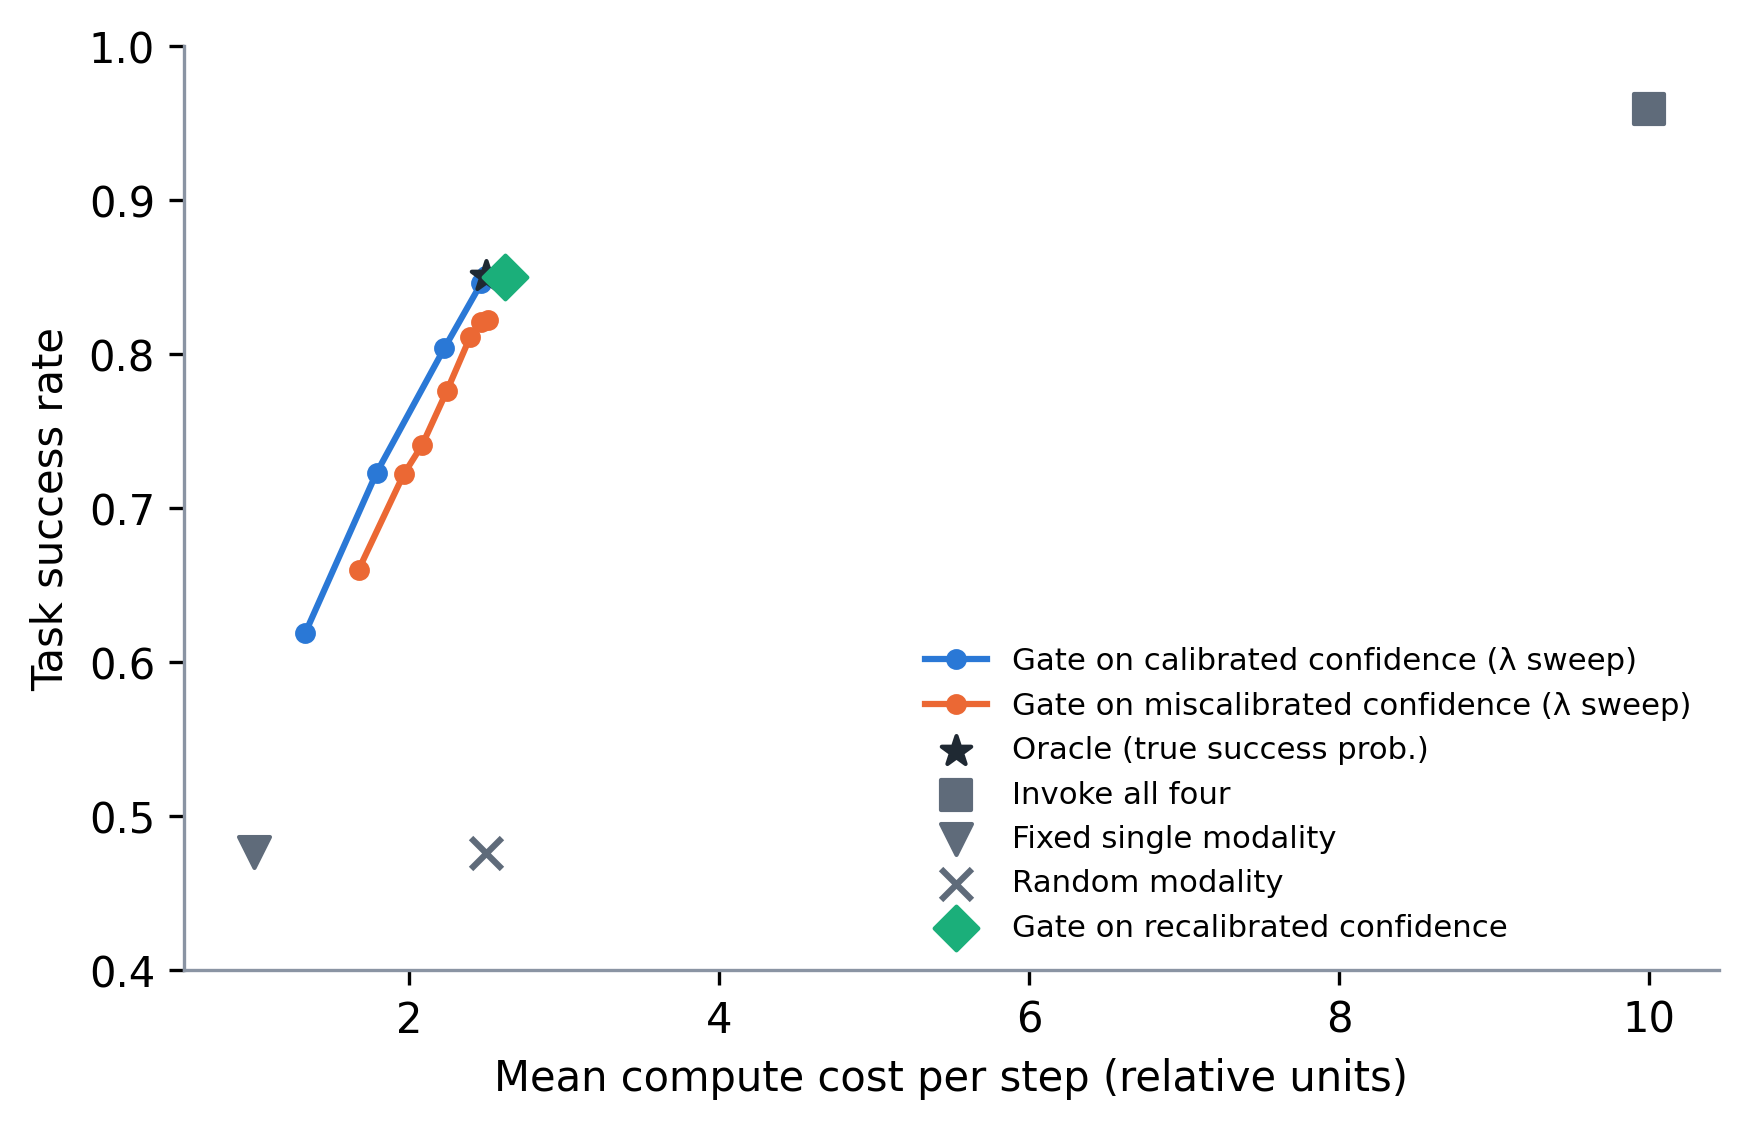
\includegraphics[width=\columnwidth]{figures/Fig4_routing_sim.png}
\caption{Illustrative simulation (not robot data): success rate against mean compute cost for confidence-gated routing among four modalities as the cost penalty \ensuremath{\lambda} varies, with calibrated (blue) and miscalibrated (orange) confidences, and baselines. Recalibration (green) coincides with the oracle. Ten seeds of 20,000 steps; standard deviations below 0.005. Code is provided as supplementary material.}\label{fig:sim}
\end{figure}


\subsection{Conditional Execution and Cascading}\label{sec:cascade}
Adaptive computation time learns how many steps to spend per input~\cite{Graves2016}, and conditional computation frames unit activation as an RL policy with a cost penalty~\cite{Bengio2015}. Cascades run a cheap model first and escalate only when needed~\cite{Chen2024,Aggarwal2024}. Fast--slow anomaly handling does the same for failures~\cite{Sinha2024}, and resource-aware reasoning learns when to invoke an LLM at all~\cite{Liu2026}. For edge orchestration, cascading suggests a default policy: run cheap perception and a fast imitation policy, and escalate to RL refinement or fault recovery only when their calibrated confidences fall below a threshold.


\subsection{Load Balancing and Expert Utilization}\label{sec:balance}
MoE training suffers from collapse onto a few experts, which auxiliary load-balancing losses counteract~\cite{Shazeer2017,Fedus2022}. In modality routing, balance is not a goal in itself, because some modalities should be rare. But collapse is still a risk: a modality that is never invoked never generates data, so its confidence is never updated. Exploration bonuses for rarely used modalities, or optimizm in the face of uncertainty, address this, following bootstrapped exploration~\cite{Osband2016}.


\subsection{The Orchestration Gap}\label{sec:position}
Fig. \ref{fig:position} positions representative works by how adaptive their orchestration is and how much they rely on calibrated uncertainty. Uncertainty-aware planners~\cite{Ren2023,Yuan2026} are calibrated but choose between acting and asking, not between learners. Routers~\cite{Ong2025,Ding2024} are learned and budget-aware but route between LLMs. Adaptive-compute VLAs~\cite{Yue2024,Zhang2026b} and adapter routers~\cite{Romer2026b,Zhu2025} route inside one model. The empty corner is a small orchestrator that is learned online on the device, uses calibrated confidences, respects a compute budget, and routes between heterogeneous learning modalities. The novelty lies in this composition, not in any single component, so any system that claims it must show that the composition performs better than its strongest parts used alone.

\begin{figure}[!t]
\centering
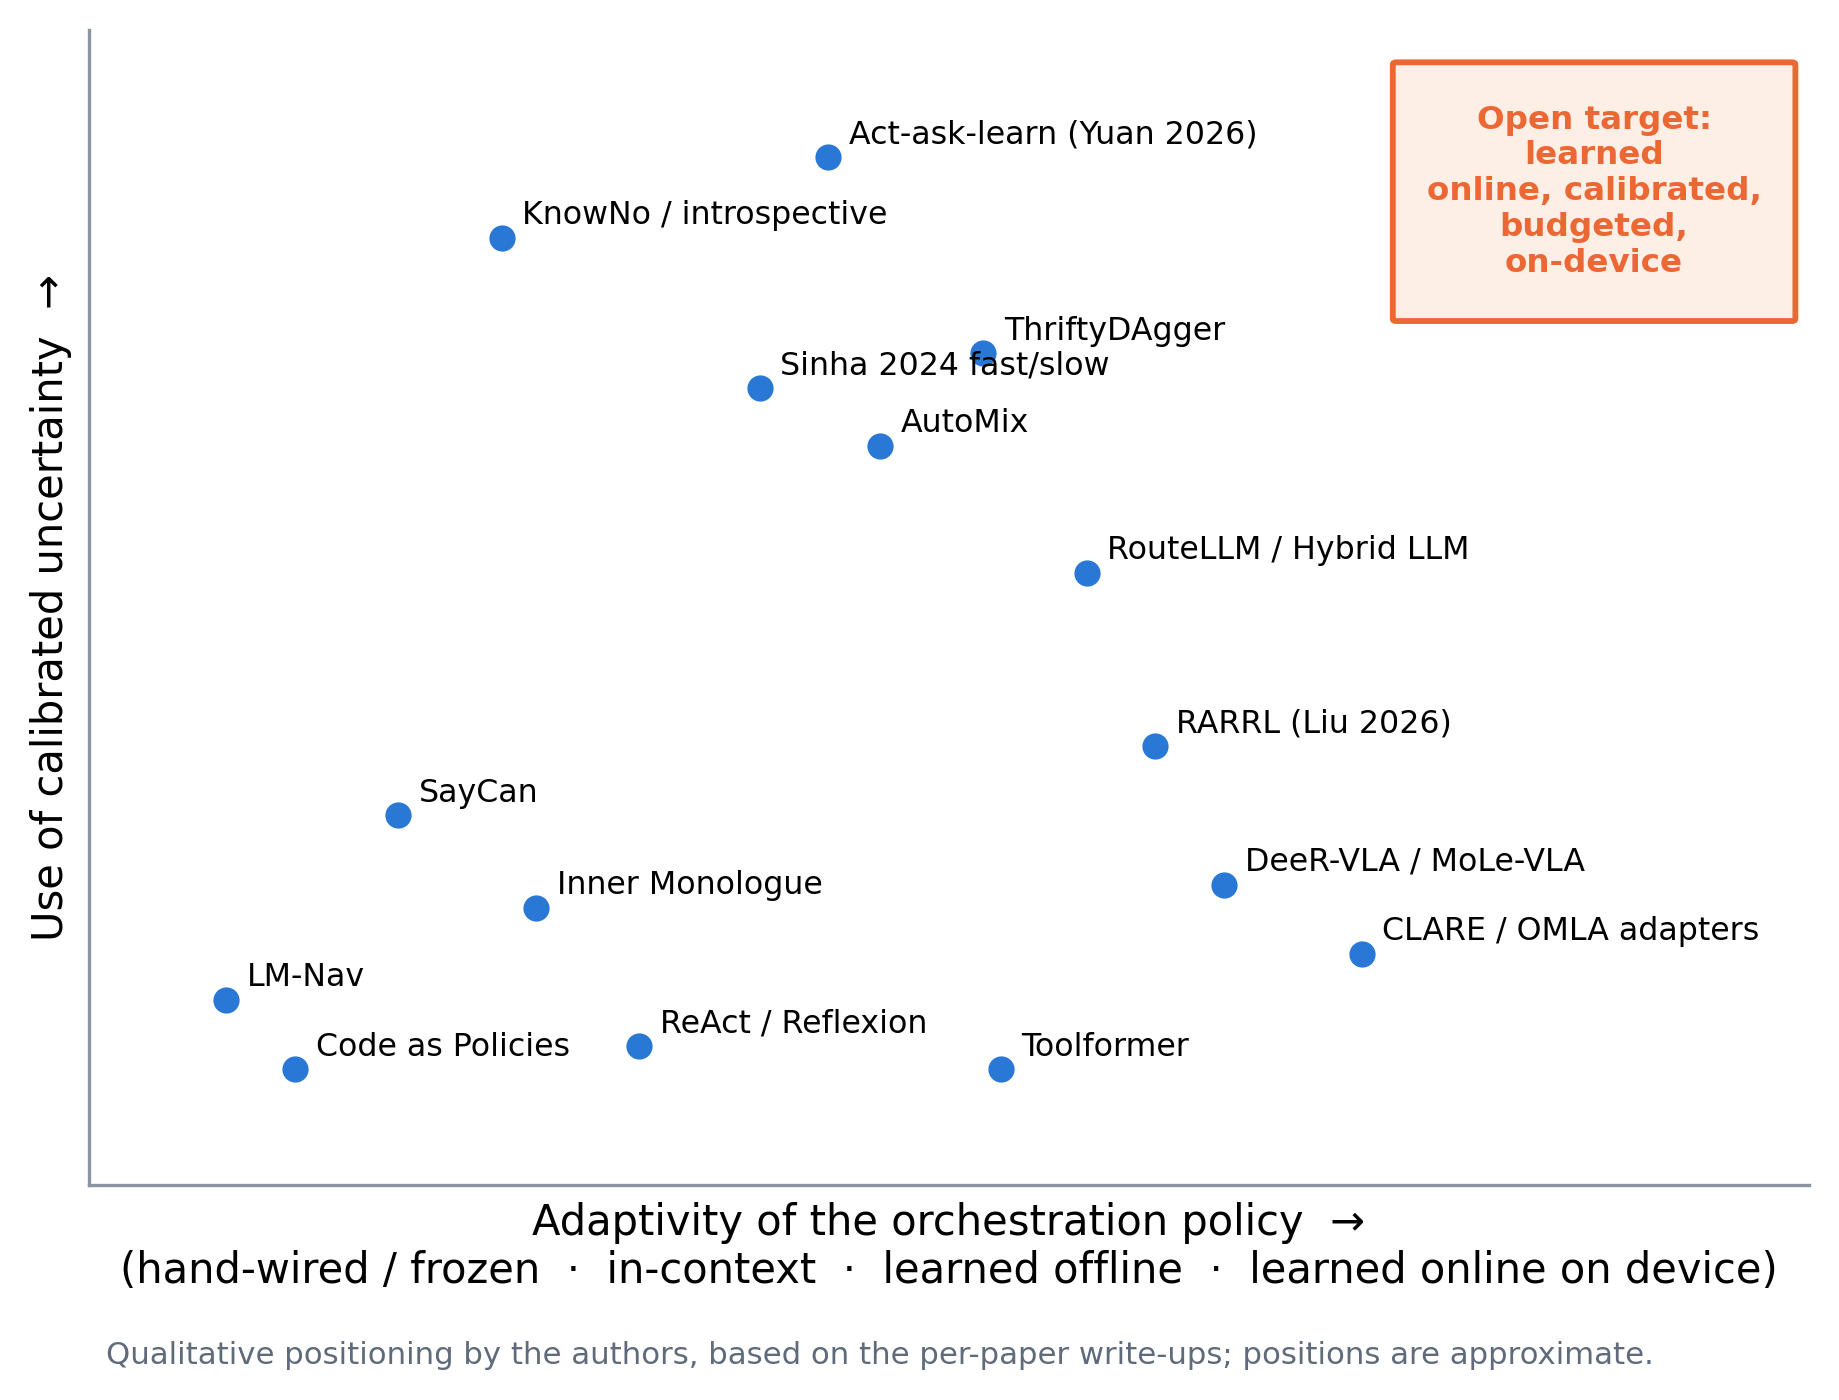
\includegraphics[width=\columnwidth]{figures/Fig5_positioning.png}
\caption{Qualitative positioning of orchestration approaches by adaptivity of the orchestration policy (horizontal) and use of calibrated uncertainty (vertical). The orange box marks the unoccupied target region. Positions are approximate and based on the per-paper write-ups.}\label{fig:position}
\end{figure}


\subsection{Formal Problem Statement}\label{sec:formal}
We propose the following formalization. At each decision step t, the agent observes context x\ensuremath{_t} (task, observation embedding, robot health) and calibrated confidences c\ensuremath{_t} = (c\ensuremath{_t}\ensuremath{^1}, \ldots{}, c\ensuremath{_t}\ensuremath{^K}) from K modalities, where c\ensuremath{_t}\ensuremath{^k} estimates the probability that invoking modality k now succeeds. The orchestrator \ensuremath{\ensuremath{\pi}\_{\ensuremath{\theta}}} selects a set S\ensuremath{_t} \ensuremath{\subseteq } {1, \ldots{}, K}, typically a single modality, incurring cost C(S\ensuremath{_t}) = \ensuremath{\Sigma}\_{k\ensuremath{\in }S\ensuremath{_t}} cost\_k and receiving task reward r\ensuremath{_t}. The objective is to maximize expected return subject to an average budget B:

\begin{equation}
\max_{\theta}\ \mathbb{E}\Big[\sum_t \gamma^t r_t\Big] \quad \text{s.t.} \quad \mathbb{E}\Big[\frac{1}{T}\sum_t C(S_t)\Big] \le B.
\end{equation}
This is a constrained Markov decision process. Its Lagrangian relaxation, maximizing E[\ensuremath{\Sigma}\ensuremath{_t} \ensuremath{\gamma}\ensuremath{^t} (r\ensuremath{_t} \ensuremath{-} \ensuremath{\lambda} C(S\ensuremath{_t}))] with \ensuremath{\lambda} \ensuremath{\geq } 0 updated by dual ascent, gives the cost-penalized gate used in Section \ref{sec:gate}. When the effect of a routing choice does not persist beyond the step, the problem reduces to a budgeted contextual bandit, where the confidences act as a learned prior over each arm's success. Three results frame what can be proved. First, if the confidences are calibrated, greedy selection of argmax\ensuremath{_k} (c\ensuremath{_t}\ensuremath{^k} \ensuremath{-} \ensuremath{\lambda} cost\ensuremath{_k}) is optimal for the one-step penalized objective. Second, miscalibration of magnitude \ensuremath{\varepsilon} in any confidence can cost at most 2\ensuremath{\varepsilon} per step in expected success relative to that optimum. Third, online calibration and exploration must be maintained for modalities that are rarely chosen (Section \ref{sec:balance}). The meta-learning view (Section \ref{sec:meta}) enters through \ensuremath{\theta}: the orchestrator is trained across a distribution of situations and adapted online by LoRA updates using replayed tuples (x\ensuremath{_t}, c\ensuremath{_t}, S\ensuremath{_t}, r\ensuremath{_t}).


\section{Low-Cost Platforms, Benchmarks, and Evaluation}\label{sec:platforms}

\subsection{A Reference Low-Cost Platform}\label{sec:lekiwi}
\textit{Hardware and compute constraints.} LeKiwi is an open-source, low-cost mobile manipulator from the LeRobot ecosystem~\cite{Cadene2026,Cadene2024}. According to its public documentation, it combines a three-wheel holonomic base with 4-inch omni wheels driven by Feetech servos and an SO-101 arm (SO-100 in earlier versions). A Raspberry Pi 5 is mounted onboard, and power comes from a 12 V battery or a 5 V power-bank variant. In the standard setup, the Pi streams observations to a laptop over ZeroMQ, where policies run. The compute constraint is therefore set by which components run on the Pi and which run on the local laptop.

\textit{Sensors.} The documented configuration has two USB RGB cameras, one viewing the workspace and one on the wrist, plus joint-position feedback from the servos. There is no depth sensor, which excludes voxel-based policies such as PerAct without additional hardware~\cite{Shridhar2022}.

\begin{table}[!t]
\centering
\caption{Documented Configuration of the LeKiwi Reference Platform}\label{tab:hw}%
\footnotesize
\begin{tabular}{@{}>{\raggedright\arraybackslash}p{0.300\dimexpr\columnwidth-4\tabcolsep\relax}>{\raggedright\arraybackslash}p{0.700\dimexpr\columnwidth-4\tabcolsep\relax}@{}}
\toprule
\textbf{Component} & \textbf{Documented configuration} \\ \midrule
Onboard computer & Raspberry Pi 5 (4 GB in the reference build) \\
Off-board computer & Laptop receiving observations over ZeroMQ \\
Base & Three-wheel holonomic drive, 4-in omni wheels, Feetech servos \\
Arm & SO-101 (SO-100 in earlier builds), with a leader arm for teleoperation \\
Cameras & Two USB RGB cameras (workspace and wrist) \\
Power & 12-V battery or 5-V power-bank variant \\
Software & LeRobot~\cite{Cadene2024,Cadene2026} \\
\bottomrule
\end{tabular}
\end{table}


\subsection{Benchmark Tasks and Task Distributions}\label{sec:bench}
Established benchmarks provide reference points but not the modality-switching structure that orchestration research needs. LIBERO~\cite{Liu2023b}, CALVIN~\cite{Mees2022}, RLBench~\cite{James2020}, Meta-World~\cite{Yu2019} and robomimic~\cite{Mandlekar2021} are simulated or fixed-arm. The task distribution should therefore be designed so that each modality is the best choice in some situations: novel objects (perception), refinable skills (RL), newly demonstrated behaviors (imitation) and induced faults such as wheel slip, payload change or camera occlusion (fault adaptation).


\subsection{Evaluation Protocol}\label{sec:protocol}
Evaluation best practice for real robots recommends pre-registered protocols, blinded or randomized trial order, reporting of all trials and confidence intervals~\cite{KressGazit2024}. Sequential testing can reduce the number of real-robot trials needed to compare two policies by up to 32\%~\cite{Snyder2025}. The large-behavior-model study shows how blinded, randomized evaluation is run at scale~\cite{TRI2025}. With about 50 trials, a success rate of 0.7 has a 95\% confidence interval of roughly \ensuremath{\pm }0.13, so differences between conditions smaller than about 0.2 will not be detectable. The trial plan should be sized with this in mind.

Following recommended practice for real-robot evaluation~\cite{KressGazit2024,Snyder2025}, each experiment should specify:

\begin{itemize}
\item Tasks and success criteria, defined before data collection.
\item Conditions (orchestrator variants and baselines) and their order, randomized across trials.
\item Fault-injection procedure and timing.
\item Number of trials per condition, chosen by power analysis or sequential testing.
\item Reset procedure and environment variation.
\item The logging needed to reproduce routing decisions (confidences, costs, selected modality, outcome).
\end{itemize}

\textit{Recommended ablations.} Each component of an orchestration system should be ablated: removing calibration so that the gate uses raw signals; using a single confidence signal instead of four; freezing the orchestrator with no LoRA updates; removing replay or the forgetting penalty; removing the compute budget (\ensuremath{\lambda} = 0); replacing the learned gate with hard-coded rules; and removing each modality in turn. Failure cases should be categorized by cause: wrong modality chosen, correct modality failed, calibration drift, or budget exhausted.


\subsection{Comparable Low-Cost Mobile Manipulation Systems}\label{sec:comparable-sys}
Mobile ALOHA~\cite{Fu2024} and Hello Robot's Stretch~\cite{Kemp2022} are the closest low-cost mobile manipulators, both with laptop- or PC-class onboard compute. ACT~\cite{Zhao2023} and SmolVLA~\cite{Shukor2025} are the policies native to the LeRobot stack, and Open X-Embodiment supplies cross-embodiment pretraining data~\cite{OXE2024}. None of these systems orchestrates learning modalities.


\section{Open Challenges}\label{sec:challenges}

\subsection{Online Calibration Across Modalities}\label{sec:ch-calib}
The central open problem is placing four heterogeneous confidence signals on one calibrated scale, and keeping it calibrated as the modalities learn and the robot changes. Conformal prediction gives distribution-free guarantees~\cite{Ren2023,Lindemann2023}, but its exchangeability assumption is broken by an orchestrator that changes which data each modality sees. Online recalibration with drift detection and evidential fusion~\cite{Han2022a} are promising directions.


\subsection{Training While Acting}\label{sec:ch-lora}
LoRA~\cite{Hu2022} and QLoRA~\cite{Dettmers2023} were designed for offline fine-tuning. Updating an orchestrator while it controls a robot raises questions of when to update, how to validate an adapter before deployment, how to avoid forgetting~\cite{Kirkpatrick2017,Rolnick2019}, and how to share the CPU with inference~\cite{Zhu2023,Cadene2026}.


\subsection{Safety of Self-Modifying Learners}\label{sec:ch-safety}
An orchestrator that retrains itself can learn unsafe routing. Safe learning in robotics~\cite{Brunke2022,Garcia2015} offers several protections. Shields synthesized from temporal logic override unsafe actions~\cite{Alshiekh2018}. The neural simplex architecture switches to a verified controller while the learner retrains~\cite{Phan2020}. Safety filters provide a unified framework~\cite{Hsu2024,Wabersich2023}. A practical design keeps a fixed, verified fallback (for example stop and ask) that the orchestrator cannot unlearn, and validates new adapters before swapping them in.


\subsection{Generalization Beyond the Task Distribution}\label{sec:ch-general}
Meta-learned orchestrators generalize only within their training distribution~\cite{Yu2019}. Novelty detection~\cite{Burda2019,Hendrycks2017} and help-seeking~\cite{Ren2023,Yuan2026} are the safeguards when the robot leaves that distribution.


\subsection{Integration With Higher-Level Planning}\label{sec:ch-plan}
The orchestrator sits below task planning. Integrating it with LLM planners~\cite{Ahn2022,Huang2022b}, so that the planner's subgoals condition modality selection and routing failures inform replanning, is a natural extension. Resource-aware reasoning shows that the decision of when to plan can itself be learned~\cite{Liu2026}.


\section{Conclusion}\label{sec:conclusion}
%CONCL
The literature supplies every ingredient of adaptive orchestration: calibrated uncertainty for perception and policies, budget-aware routing, adaptive computation, parameter-efficient continual learning, and runtime failure detection. What it lacks is their composition into a learned arbiter over heterogeneous learning modalities on edge hardware.

Treating the orchestrator as a meta-learner that routes on calibrated confidences under a budget unifies MoE, cascades and meta-RL in one formulation (Section \ref{sec:formal}). The illustrative simulation shows that calibration is not optional: routing inherits every calibration error.

If the claims hold, low-cost robots could adapt continuously without cloud connectivity, which matters for privacy, latency, cost and robustness. The survey's evidence suggests that this is achievable with small models and careful calibration, and that the main risks lie in calibration drift and the safety of self-modifying learners.


\section*{Acknowledgment}
\fillin{acknowledgments and funding, or delete this section}


\appendices

\section{Mathematical Details}\label{app:math}

\subsection{Budgeted Routing as a Constrained MDP}\label{app:cmdp}
With state s\ensuremath{_t} = (x\ensuremath{_t}, c\ensuremath{_t}, b\ensuremath{_t}), where b\ensuremath{_t} is the remaining budget, action S\ensuremath{_t}, reward r\ensuremath{_t} and cost C(S\ensuremath{_t}), the Lagrangian L(\ensuremath{\theta}, \ensuremath{\lambda}) = E[\ensuremath{\Sigma}\ensuremath{_t} \ensuremath{\gamma}\ensuremath{^t} (r\ensuremath{_t} \ensuremath{-} \ensuremath{\lambda} C(S\ensuremath{_t}))] + \ensuremath{\lambda}B is maximized over \ensuremath{\theta} and minimized over \ensuremath{\lambda} \ensuremath{\geq } 0. A practical algorithm alternates policy-gradient updates of \ensuremath{\theta} (for example PPO~\cite{Schulman2017}) with the dual update \ensuremath{\lambda} ← max(0, \ensuremath{\lambda} + \ensuremath{\eta } (Ĉ \ensuremath{-} B)).


\subsection{One-Step Optimality Under Calibration}\label{app:opt}
If c\ensuremath{^k} = P(success | k, x) exactly, the expected penalized reward of choosing k is c\ensuremath{^k} \ensuremath{-} \ensuremath{\lambda} cost\ensuremath{_k}, so argmax\ensuremath{_k} (c\ensuremath{^k} \ensuremath{-} \ensuremath{\lambda} cost\ensuremath{_k}) is optimal for the one-step objective. If each reported confidence differs from the truth by at most \ensuremath{\varepsilon}, the chosen arm's true value is within 2\ensuremath{\varepsilon} of the optimum. This bound motivates the calibration step.


\subsection{Calibration Maps}\label{app:calib}
Temperature scaling divides logits by T fitted by maximum likelihood on held-out data~\cite{Guo2017}. Platt scaling fits \ensuremath{\sigma}(a\ensuremath{\cdot }s + b) to a raw score s~\cite{Zollo2025}. For the simulation we fitted a linear map from reported confidence to observed success per modality. Split conformal prediction chooses the threshold \ensuremath{\hat{q}} as the \ensuremath{\lceil }(n+1)(1\ensuremath{-}\ensuremath{\alpha})\ensuremath{\rceil }/n quantile of calibration scores, which gives coverage of at least 1\ensuremath{-}\ensuremath{\alpha} under exchangeability~\cite{Ren2023}.


\subsection{Recovery-Success Posterior}\label{app:beta}
With a Beta(\ensuremath{\alpha}\ensuremath{_0}, \ensuremath{\beta}\ensuremath{_0}) prior and s successes in n recovery attempts for a fault class, the posterior mean (\ensuremath{\alpha}\ensuremath{_0} + s)/(\ensuremath{\alpha}\ensuremath{_0} + \ensuremath{\beta}\ensuremath{_0} + n) is the fault modality's confidence, and its variance measures how much that confidence can be trusted.


\subsection{A Candidate Orchestrator Update Algorithm}\label{app:alg}
\begin{itemize}
\item Observe x\ensuremath{_t}; query the calibrated confidences c\ensuremath{_t} from the four modalities (cheap signals every step, expensive ones on demand).
\item Select S\ensuremath{_t} = argmax\ensuremath{_k} \ensuremath{\ensuremath{\pi}\_{\ensuremath{\theta}}}(k | x\ensuremath{_t}, c\ensuremath{_t}, b\ensuremath{_t}), subject to the fallback shield (Section \ref{sec:ch-safety}).
\item Execute; record (x\ensuremath{_t}, c\ensuremath{_t}, S\ensuremath{_t}, r\ensuremath{_t}, outcome) in the replay buffer.
\item Periodically, in the background: recalibrate each modality's confidence map on recent outcomes; update the LoRA adapter of \ensuremath{\ensuremath{\pi}\_{\ensuremath{\theta}}} on prioritized replay~\cite{Schaul2016} with a forgetting penalty~\cite{Kirkpatrick2017}; validate the new adapter on held-out episodes before swapping it in; update \ensuremath{\lambda} by dual ascent.
\end{itemize}


\section{Illustrative Routing Simulation: Full Results}\label{app:sim}
Table \ref{tab:simres} reports the illustrative simulation of Section \ref{sec:gate}. The data are synthetic; no robot experiments were run for this survey. The simulation code is provided as supplementary material.

\begin{table}[!t]
\centering
\caption{Illustrative Routing Simulation: Success Rate and Mean Compute Cost (\ensuremath{\lambda} = 0.05), Mean \ensuremath{\pm } SD Over 10 Seeds of 20 000 Steps (Synthetic Data)}\label{tab:simres}%
\footnotesize
\begin{tabular}{@{}>{\raggedright\arraybackslash}p{0.500\dimexpr\columnwidth-6\tabcolsep\relax}>{\raggedright\arraybackslash}p{0.250\dimexpr\columnwidth-6\tabcolsep\relax}>{\raggedright\arraybackslash}p{0.250\dimexpr\columnwidth-6\tabcolsep\relax}@{}}
\toprule
\textbf{Policy} & \textbf{Success rate} & \textbf{Mean cost per step} \\ \midrule
Oracle (true success prob.) & 0.851 \ensuremath{\pm } 0.003 & 2.5 \\
Invoke all four & 0.959 \ensuremath{\pm } 0.001 & 10.0 \\
Fixed single modality & 0.477 \ensuremath{\pm } 0.005 & 1.0 \\
Random modality & 0.476 \ensuremath{\pm } 0.004 & 2.5 \\
Gate on calibrated confidence & 0.851 \ensuremath{\pm } 0.003 & 2.5 \\
Gate on miscalibrated confidence & 0.811 \ensuremath{\pm } 0.004 & 2.4 \\
Gate on recalibrated confidence & 0.850 \ensuremath{\pm } 0.003 & 2.5 \\
\bottomrule
\end{tabular}
\end{table}

Sweep of the cost penalty \ensuremath{\lambda} (success rate, mean cost), calibrated gate: \ensuremath{\lambda} = 0: 0.851, 2.50; \ensuremath{\lambda} = 0.02: 0.851, 2.50; \ensuremath{\lambda} = 0.05: 0.851, 2.50; \ensuremath{\lambda} = 0.1: 0.846, 2.47; \ensuremath{\lambda} = 0.15: 0.804, 2.23; \ensuremath{\lambda} = 0.2: 0.723, 1.79; \ensuremath{\lambda} = 0.3: 0.619, 1.33. Miscalibrated gate: \ensuremath{\lambda} = 0: 0.822, 2.51; \ensuremath{\lambda} = 0.02: 0.821, 2.46; \ensuremath{\lambda} = 0.05: 0.811, 2.39; \ensuremath{\lambda} = 0.1: 0.776, 2.24; \ensuremath{\lambda} = 0.15: 0.741, 2.08; \ensuremath{\lambda} = 0.2: 0.722, 1.97; \ensuremath{\lambda} = 0.3: 0.660, 1.68.


\bibliographystyle{IEEEtran}
\bibliography{refs}

%% Biographies (IEEE Transactions require them; photos optional at submission)
\begin{IEEEbiographynophoto}{Firstname Lastname}
\fillin{biography (education, current position, research interests)}
\end{IEEEbiographynophoto}

\begin{IEEEbiographynophoto}{Second Author}
\fillin{biography}
\end{IEEEbiographynophoto}

\end{document}
